\documentclass{tnreport}
%\documentclass[confidential]{tnreport} % If you are writing confidential report

\def\reportTitle{Support de la modélisation solide dans l'impression 3D : Évaluation au travers du format AMF} % Titre du mémoire
\def\reportLongTitle{Support de la modélisation solide dans l'impression 3D : Évaluation au travers du format AMF} % Titre plus long du mémoire

\def\reportAuthor{Virgile Daugé}
\def\reportAuthorEmail{\email{virgile.dauge@telecomnancy.net}} % Courriel de l'élève

\def\reportAuthorAddress{1, rue du Général de Castelnau} % Adresse de l'élève
\def\reportAuthorCity{54600, Villers-lès-Nancy} % Adresse (cont.) de l'élève
\def\reportAuthorPhone{t+33 6 63 46 19 65} % Téléphone de l'élève 

\def\reportIndustrialSupervisor{Jean-François Rotgé} % Prénom Nom de l'encadrant industriel
\def\reportAcademicSupervisor{Thibault Cholez} % Prénom Nom de l'encadrant académique

\def\reportCompany{Parallel Geometry} % Nom de l'entreprise d'accueil
\def\reportCompanyAddress{400, ave Atlantic Bureau 100}  % Adresse de l'entreprise
\def\reportCompanyCity{H2VlA5, Outremont, Canada} % Adresse (cont.) de l'entreprise
\def\reportCompanyPhone{+1 (514) 277-6413} % Téléphone de l'entreprise
\def\reportCompanyLogoPath{figures/llg} % Logo de l'entreprise -- comment this definition to remove company logo

\def\place{Montréal} % Ville pour la signature pour l'engagement anti-plagiat
\def\date{\today} % Date pour la signature de l'engagement anti-plagiat


\begin{document}
  
\maketitle
\pagenumbering{roman}

\insertAntiPlagiarismAgreement{Daugé, Virgile}{31110541}

\cleardoublepage

\makesecondtitle

\section*{Remerciements}
\addcontentsline{toc}{chapter}{Remerciements}

{\em
J'adresse mes remerciements aux personnes qui m'ont aidé dans la réalisation de ce stage.

En premier lieu, je remercie Mr Denis Akzam, CEO de Parallel Gometry pour son accueil au sein de l'entreprise.

Je remercie également Jérémie Farret pour le temps qu'il m'a consacré, le suivi constant apporté ainsi que ses conseils avisés aidant au bon déroulement du stage.

Je tiens enfin à remercier Jean-François Rotgé pour son aide théorique, ainsi que pour de nombreux échanges enrichissants, qui m'ont permis d'appréhender des concepts nouveaux et prometteurs. 
}

\hspace{4cm}

\cleardoublepage

\renewcommand{\baselinestretch}{0.5}\normalsize
\tableofcontents
\renewcommand{\baselinestretch}{1.0}\normalsize
\cleardoublepage

\pagenumbering{arabic}
\setcounter{page}{1}

\chapter{Introduction}
La fabrication additive a connu une croissance exponentielle ces dernières années, autant par la multiplication des domaines d'activités que par l'explosion des capacités des imprimantes. De nombreux standards définissent des formats de fichiers aux utilisations diverses dans le monde de la fabrication additive. Néanmoins, une grande partie du secteur utilisait, et utilise toujours le format de fichier assez pauvre baptisé STL\footnote{STL vient de Stéréolitographie.}. Il devenait alors évident qu'un nouveau format devait être standardisé afin de suivre au mieux les nécessités et les capacités grandissantes du domaine. 

C'est dans ce contexte que l'organisation internationale de normalisation (ISO) ainsi que l'American Society for Testing and Materials (ASTM) ont collaboré pour créer la norme AMF pour additive manufacturing File Format, qui est aujourd'hui la norme internationale pour l'impression 3D. La norme AMF est un standard de fichiers couvrant les besoins actuels et futurs de la fabrication additive. Elle vient remplacer l'ancien mais toujours très utilisé fichier STL, en apportant une compression supérieure permettant de gagner sur le volume nécessaire au stockage. Ce gain de place a fait le succès de ce format de fichier, néanmoins ce n'est qu'une de ses caractéristiques prometteuses. Comme en STL, l'objet est représenté par sa surface, sous forme de meshs\footnote{un mesh, ou maillage, est une modélisation géométrique par des éléments bien définis, souvent des triangles.} composés d'assemblages de triangles. Autre nouveauté apportée par la norme AMF, la gestion de matériaux, et par extension, de couleurs. C'est là le principal atout de cette norme, quoique peu utilisé à l'heure actuelle, certainement par manque de connaissances et de documentations.

La mise à jour de la norme AMF n'était pas au goût du jour, jusqu'à ce qu'un nouveau consortium fasse sont entrée, 3MF, poussant un format éponyme, qui partage de nombreux points communs avec AMF, sur le devant de la scène. Il devint alors nécessaire pour les organismes gérant la norme AMF de la mettre à jour, pour conserver une certaine compétitivité et ainsi assurer la pérénité de la norme. Malheureusement, les initiateurs et principaux acteurs du projet, à savoir Jonathan Hiller et Hod Lipson, ne sont plus actifs à ce jour. Cela a pour conséquence une méconnaissance des possibilités d'AMF et de son logiciel de référence, AMFTools. Il s'avère donc nécessaire pour le groupe de travail de la norme de faire le point sur les capacités de la norme en l'état, avant de songer à y apporter des modifications.

C'est là qu'intervient ce stage, ayant pour but de cerner aux mieux les possibilités offertes actuellement par le Couple AMF AMFTools, en particulier les possibilités de représentations solides. En effet, l'équipe de Parallel Geometry, experte dans le domaine, y entrevoit une possibilité de démontrer les inconvénients de la représentation polygonale actuellement utilisée, et par extension les bénéfices de la représentation solide, ou mieux encore de l'arithmétique des formes.    

L'objectif est donc dans un premier temps la réalisation d'une batterie de tests complets permettant d'illustrer les différentes fonctionnalités prévues par la norme, afin d'identifier les limites actuelles et proposer d'éventuels axes d'amélioration de la norme.
\cleardoublepage

\chapter{Présentation de l'entreprise}
Ce stage s'effectue à Montréal, au sein de l'entreprise P4BUS\footnote{Plus d'informations ici: \url{http://p4bus.com/}}, filiale de Parallel Geometry\footnote{Plus d'informations ici: \url{http://llgeometry.com/}} dédiée à l'exploitation des innovations et des brevets de Parallel Geometry, et plus particulièrement ceux s'appliquant à la fabrication additive. Ces innovations sont le fruit d'une recherche incessante menée par Jean-François Rotgé, dans la continuité de sa thèse sur l'arithmétique des formes, présentée dans la sous-section \ref{subsec:arithform}. Le groupe est en réalité une petite équipe aux compétences complémentaires. Bien qu'étant une petite entreprise comptabilisant moins de 10 employés, Parallel Geometry détient un savoir faire unique au monde, demandé par de nombreuses multinationales. Ils ont ainsi eu l'occasion de travailler en partenariat avec Intel ou encore l'agence Spaciale Canadienne sur de la simulation parallèle. En effet, bien que la 3D soit le coeur de métier de LLG, leur confortable avance dans de nombreux domaines de l'algorithmique leur permet d'apporter une réelle aide à ces grandes entités. Dans le cadre de la robotique cette fois, ils ont effectué en collaboration avec l'agence spaciale Canadienne des simulations de collision, ainsi que de dynamiques de contact sur bras robotisé équipant actuellement la station spaciale internationale. Des acteurs importants du domaine de l'informatique, comme Dassault Systèmes, font également appel à Parallel Geometry lorsqu'ils se retrouvent en difficulté face à un algorithme particulier. Effectuer mon stage au sein de cette entreprise représente donc pour moi une réelle opportunité, ainsi qu'un fort enrichissement personnel. 

\cleardoublepage

\chapter{Découverte}

Mes connaissances dans le domaine de la modélisation 3D ainsi que dans l'impression 3D ont nécessité une mise à jour, dans l'objectif d'être capable de cerner au mieux les concepts et enjeux abordés dans le contexte du stage. De nombreuses documentations et recherches ont par ce fait été menées, et ce tout au long du stage. Ces différents travaux sont évoqués dans leur contexte spécifique, permettant ainsi au lecteur néophyte d'aborder sereinement chaque test. Néanmoins, un travail de fond a été effectué lors de la première semaine de stage, sur différents points décrits ci-dessous. 

\section{Géometrie constructive et modélisation solide}\label{sec:csg}
Les représentations dites solides\footnote{Constructive solid geometry (CSG) en anglais} font partie d'une branche de la modélisation numérique d'objets, à travers leurs définitions géométriques. Un objet est défini par une combinaison d'opérations sur des objets primitifs tels le cube ou la sphère. Les opérations possibles sont d'une part booléennes : l'union, l'intersection et la différence, et d'autre part des transformations géométriques : translation, rotation, homothétie. On stocke la combinaison d'opérations sous la forme d'un arbre, comme l'illustre la figure suivante. 
\begin{figure}[ht]
  \centering
  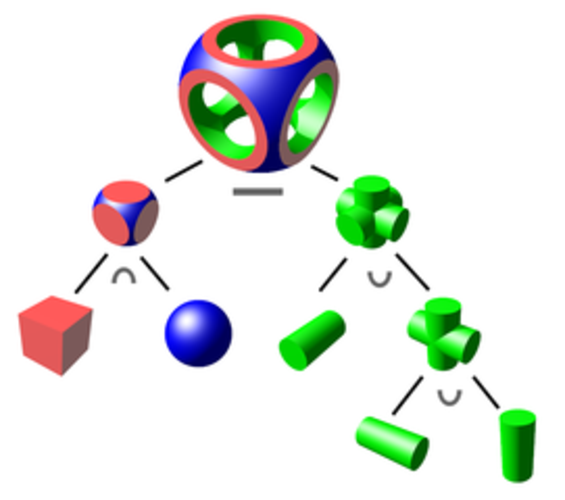
\includegraphics{figures/csg_tree}
  \caption{Arbre d'opérations}
  \label{fig:csg_tree}
\end{figure}
Il est donc possible de définir n'importe quel objet de cette manière, toutefois des objets aux formes complexes peuvent aisément demander de très nombreuses opérations et ainsi alourdir un peu les calculs de rendu. De plus, il n'est pas forcément évident de décomposer l'objet que l'on cherche à représenter, ce qui peut limiter les possibilités de création.

Malgré ces points, cette technique de modélisation propose d'incontournables avantages par rapport à la technique la plus répandue actuellement : la représentation polygonale. Premièrement, les techniques à base de polygones se contentent d'approximer la surface réelle de l'objet, nécessitant de nombreux polygones pour obtenir un résultat visuellement convaincant. La géométrie constructive détient, quant à elle, une définition exacte de l'objet à travers sa formulation mathématique. Autre point important, particulièrement dans le monde de l'impression 3D, l'information de l'intérieur du volume est également stockée. On a ainsi une définition à la fois complète et exacte de l'objet. De plus, les calculs sont largement simplifiés avec cette représentation, qu'il s'agisse de l'intersection avec une droite comme pour le ray tracing ou de projections de formes dans le cas de l'ombrage. Le calcul de collisions devient instantané dans des configurations simples, puisqu'il est possible d'évaluer directement les points que les solides ont en commun. Les gains en volume mémoire sont également impressionnants. En effet, si l'on prend par exemple les deux sphères qui seront utilisées lors de tests ultérieurs, l'espace de stockage nécessaire en polygones est de 1.2Mo, pour un résultat très approximé, dont les facettes sont visibles à l'oeil nu, contre moins d'1Ko en modélisation solide, pour une définition exacte. 
\subsection{Arithmétique des formes}
\label{subsec:arithform}
L'arithmétique des formes est un langage universel volumique, permettant la description arithmétique des formes. Elle s'appuie sur les mathématiques pour résoudre des problématiques complexes et ainsi proposer une manière efficace de stocker et transmettre l'information volumique, évitant les excès d'espace mémoire et de temps de calculs réclamés par la représentation polygonale. Le caractère universel de ce langage est basé sur les concepts suivants, énoncés par Jean-François Rotgé dans un acte de conférence :
\begin{itemize}
    \item Portabilité et indépendance vis à vis du contexte d'utilisation
    \item Unification qui assure une résolution générale des problématiques géométriques à l'aide d'une algorithmique sans cas particuliers
    \item Pérénité assurant la validité du langage dans le temps
    \item Interoptabilité qui assure les futures évolutions contextuelles
    \item Adaptibilité qui assure les futures évolutions contextuelles
    \item Compatibilité qui assure l'immigration de l'information déjà disponible
\end{itemize}
Cette théorie a été inspirée par les travaux de Monge, notamment sa Géométrie Descriptive (1800), ainsi que par l'Algèbre Ornementale de Maurice El-Millick (1936). Sa force est d'intégrer la théorie géométrique fortement abstraite de construction de volumes, le langage topologique. Cela par la transmutation de la problématique topologique et géométrique en problématique logique et arithmétique permettant par la suite de simplifier stockage de l'information et calculs, tout en conservant l'exactitude des résultats.

L'arithmétique des formes englobe la représentation CSG définie auparavant, en corrigeant les problèmes de cette dernière. En effet, les opérations binaires ne sont pas suffisantes pour définir un objet, on est limité à l'état d'appartenance ou non à un objet. Cela a pour conséquence certaines erreurs classiques comme l'effet de peau/pellicule, survenant lorsque l'on fait la différence entre deux objets ayant une surface coïncidente. Ces effets entretiennent une habitude de corruption volontaire des données afin d'obtenir le résultat attendu. Dans cet exemple, il est commun d'étendre l'objet à soustraire pour le faire dépasser de l'objet auquel on le soustrait et ainsi supprimer la zone ambiguë. En arithmétique des formes, les opérateurs N-aires\footnote{Opérateurs à N dimensions, les opérateurs binaires n'en possédant que deux.} permettent de corriger cela.

L'arithmétique des formes ne sera plus abordée directement lors de ce rapport, mais certains des tests effectués permettront à tous de comprendre la richesse des possibilités offertes par l'arithmétique des formes. Il est difficile d'envisager, du point de vue curieux et intéressé d'un étudiant, les raisons pour lesquelles la représentation polygonale, qui parait préhistorique, tant dans sa conception que dans ses capacités, est toujours prédominante.
\section{Formats de fichiers}
Il est indispensable d'avoir une connaissance au moins globale des formats de fichiers existants pour pouvoir travailler convenablement sur l'un d'entre eux. C'est dans cette optique qu'est proposée cette section. 
\subsection{STL}
Le format de fichier STL a été développé par la société 3D Systems. C'est un format de fichiers stockant un objet 3D. Seule la surface de l'objet y est stockée à travers une approximation triangulaire. Son niveau sémantique est très bas, on y définit chaque triangle composant la surface de l'objet représenté, comme l'illustre le listing suivant, qui définit un objet composé d'un seul triangle. 
\lstinputlisting[caption={Syntaxe STL}]{src/stl_example.stl}
Il s'agit bien entendu d'une représentation polygonale, aussi populaire que pauvre en termes de contenu. On devra donc se contenter de l'information de surface, sans couleurs ni définitions de matériaux et même sans unité. Si cela peut sembler léger pour une représentation 3D, ça l'est encore plus quand il s'agit d'imprimer un objet ainsi défini. On peut également noter qu'avec un standard de stockage similaire, la taille d'un fichier dépend intimement de la taille de l'objet à représenter, ainsi que de son niveau de détail. 
\newpage
\subsection{Additive Manufacturing File Format}
Après un rapide bilan des possibilités limitées du format STL face aux capacités croissantes des imprimantes 3D, on comprend la nécessité d'établir un nouveau standard de fichiers. L'organisation internationale de normalisation (ISO) ainsi qu'ASTM International ont travaillé de concert sur la conception du successeur de STL, l'Additive Manufacturing File Format (AMF). Les grandes lignes directrices d'AMF sont les suivantes:
\begin{enumerate}
  \item Indépendant de la technologie
  \item Simplicité
  \item Evolutivité
  \item Performances
  \begin{enumerate}
    \item Rapidité de lecture et d'écriture
    \item Taille de fichier raisonnable
  \end{enumerate}
  \item Rétrocompatibilité avec STL (Avec perte des données suplémentaires)
  \item Extensibilité
\end{enumerate}
AMF est un format basé sur XML, apportant des solutions à certaines lacunes évoquées précédemment. AMF propose ainsi un support natif de la couleur, des matériaux, de la structure interne de l'objet à travers de lattices, ainsi que des constellations permettant de définir plusieurs objets accompagnés de leurs coordonnées dans l'espace au sein d'un même fichier AMF. Les méta-données sont également possibles, mais leur utilisation n'est pas normée. AMF propose aussi la possibilité de définir l'unité de mesure utilisée. 

\subsubsection{Syntaxe}
La syntaxe d'AMF est assez simple, on commence par définir un ou plusieurs objets, contenant une liste de points ainsi qu'un ou plusieurs volumes. Un volume est composé de triangles définis par trois points de la liste précédente. Le listing \ref{lst:AMFexample} est le code AMF de l'exemple énoncé. 
\lstinputlisting[language=AMF, caption={Exemple d'AMF}, label={lst:AMFexample}]{src/amf_example.amf}
On peut assigner une couleur et un matériau à un volume, définissant respectivement la couleur de la surface et la composition de l'objet comme l'illustre le listing \ref{lst:matassign}. Le matériau doit être défini dans le même fichier.
\begin{lstlisting}[language=AMF,caption={Assignation de couleur et matériau à un volume}, label={lst:matassign}]
<volume materialid="1">
        <color>
          <r>0.8</r>
          <g>0.8</g>
          <b>0.8</b>
        </color>
\end{lstlisting}
La notion de matériau est importante, c'est elle qui permet de définir toute la structure interne de l'objet. Un matériau se définit au même niveau que l'objet. Le listing \ref{lst:defmat} indique la syntaxe de définition d'un matériau.
\begin{lstlisting}[language=AMF,caption={Définition de matériau},label={lst:defmat}]
<material id="1">
    <metadata type="name">Materiau A</metadata>
    <color>
      <r>0.8</r>
      <g>0.5</g>
      <b>0.4</b>
    </color>
</material>
\end{lstlisting}
\subsubsection{Optimisations}
Comme évoqué précédemment, AMF stocke une liste de points, avant de les assigner aux triangles. Cela permet de ne définir qu'une seule fois chaque point, contrairement à STL qui les redéfinit pour chaque triangle. Cela apporte deux avantages, le premier, évident, est une réduction de la taille des données. Le second permet de corriger les erreurs d'ajustements entre triangles de manière native. En STL, cette correction était attribuée aux algorithmes de slicing, chargés de découper l'objet 3D en tranches 2D.
\subsection{3MF}
Le format 3MF est très similaire à AMF, mais il est supporté par un consortium industriel mené par Microsoft (3MF Consortium). Il est nativement supporté par windows 10. 3MF ne fait pas l'objet du stage, mais il en est à l'origine. En effet, c'est l'arrivée de ce concurrent direct à AMF qui a poussé le groupe de travail d'AMF à faire le point sur les capacités actuelles d'AMF. Cela dans le but de pouvoir l'améliorer, et ainsi satisfaire de nouveaux utilisateurs potentiels, tout particulièrement demandeurs sur la représentation solide. 
\subsection{Autres}
Il existe de très nombreux autres formats, la liste de ceux étudiés lors de ce stage est disponible dans le tableau \ref{tab:fichiers}.\\

\begin{tabular}{|m{2cm}|m{4cm}|m{7cm}|}
\label{tab:fichiers}
   Format & technologie & commentaires\tabularnewline
   \hline
   X3D & polygones & Format prévu pour le web, il contient des informations inutiles pour l'impression comme le son ou l'animation \tabularnewline
   \hline
   STEP & modélisation solide & Il est peu utilisé dans la fabrication additive\tabularnewline
   \hline
   PLY & polygones & Utilisé pour les données de scanners 3D, support de la couleur\tabularnewline
   \hline
   OBJ & polygones & Simple, très utilisé, support de texture mais pas de matériaux\tabularnewline
   \hline
   3DS & polygones & Limité à 65636 triangles, support de la texture\tabularnewline
   \hline
   ACIS & polygones + modélisation solide & Orienté objet. Très utilisé en conception assistée par ordinateur\tabularnewline
   \hline
\end{tabular}
\cleardoublepage



\chapter{Audit}

Il s'agit ici du coeur du travail réalisé au sein du stage, son objectif étant de cerner les possibilités actuelles du couple AMF/AMFTools. Et ce plus particulièrement concernant la représentation du solide. Pour répondre à ces problématiques, il s'est avéré nécessaire d'adopter plusieurs approches, décrites dans la suite de ce chapitre.

AMFTools est le logiciel open source de référence accompagnant la norme AMF. Il a été développé par Jonathan Hiller. Il comporte déjà de nombreuses fonctionnalités, dont la liste est énoncée sur le wiki d'AMF \cite{AMFwikispacessoft}. Voici les fonctionnalités incluses dans la version 0.9.7 :
\begin{itemize}
  \item Visualisation et manipulations 3D 
  \item Imports de fichiers STL
  \item Imports limités de fichiers X3D 
  \item Création et édition des Constellations
  \item Création, édition et assignement de matériaux à un objet
  \item Support des équations de répartitions de matériaux à l'intérieur de l'objet
  \item Vue en coupe de l'objet 3D
  \item Support des triangles curvilignes
  \item Interface utilisateur améliorée, avec un accès plus direct aux fonctionnalités.
\end{itemize}

\section{Boîte blanche}
L'approche boite blanche signifie bien entendu une analyse du code d'AMFTools. Celle-ci s'est avérée nécessaire au début de l'étude globale. En effet, la prise en charge de la modélisation solide par le couple AMF/AMFTools n'étant pas clairement délimitée, la documentation fournie et les exemples mis à disposition des utilisateurs ne permettent pas de créer des fichiers d'exemples. Il est également toujours profitable de connaître le fonctionnement de l'outil que l'on cherche à évaluer.  
\subsection{Recherche d'éléments concernant la gestion du solide}
\label{subsec:elementsolides}
Après un rapide survol du code, il s'est avéré que le support de la modélisation solide n'était pas supporté en tant que tel. Il reste indispensable en AMF d'utiliser un mesh pour décrire la surface du volume. L'objectif de cette sous-section est de montrer les méthodes de recherche choisies ainsi que de présenter les pistes pour les tests ultérieurs. 
\subsubsection{Libraire MuParser}

La présence d'un dossier "MuParser" dans la racine du projet est un début de piste sur le support des lattices et de la représentation fonctionnelle de la structure interne de l'objet. En effet, Muparser est une librairie C++ de parsing d'équations mathématiques, comme l'explique en détail son site \cite{muparsersite}. Or la représentation fonctionnelle de l'intérieur de l'objet est une des seules parties d'AMF utilisant potentiellement des équations mathématiques. 

\subsubsection{Traces d'équations}\label{subsec:tracequa}
Par la suite, l'utilisation de l'outil de recherche avancé de SublimeText 3\footnote{SublimeText est un éditeur de texte très complet} a permis d'identifier rapidement 7 fichiers dans lesquels il est question d'équations.

Les deux premiers fichiers mentionnés sont Amf.cpp et "Amf\_file.cpp", il est question ici à la fois d'équations de mise à l'échelle, qui ne nous concernent pas, et des méthodes permettant de récupérer l'équation d'un composite. Ce qui représente une piste prometteuse.

Le fichier Equation.cpp a tout particulièrement attiré mon attention. Il gère toutes les équations, y compris les équations de mise à l'échelle, mais la partie qui nous intéresse ici se situe dans le parser de l'équation. Plus précisément dans la fonction IniParser(), disponible sur le listing \ref{lst:parserequation}. On peut constater ici que les équations sont prévues pour contenir des opérations spécifiques à la représentation fonctionnelle : mod, and, or, xor... On remarque également que seules trois variables sont définies, x,y et z. On peut en déduire que la structure interne peut être définie ici en fonction de la position dans l'objet. Nous y sommes, la représentation fonctionnelle est supportée dans la version actuelle d'AMFTools. Reste encore à déterminer à quel niveau elle est implémentée. 

\begin{lstlisting}[language=c++, caption={parser d'équations}, label={lst:parserequation}]
void CEquation::IniParser()
{
	if (!pP){ //if not already initialized...
		pP = new mu::Parser;

		pP->DefineOprt("%", CEquation::Mod, 6); //deprecated
		pP->DefineFun("mod", &CEquation::Mod, false);
		pP->DefineOprt("&", AND, 1); //DEPRECATED
		pP->DefineOprt("and", AND, 1);
		pP->DefineOprt("|", OR, 1); //DEPRECATED
		pP->DefineOprt("or", OR, 1);
		pP->DefineOprt("xor", XOR, 1);
		pP->DefineInfixOprt("!", NOT);
		pP->DefineFun("floor", &CEquation::Floor, false);
		pP->DefineFun("ceil", &CEquation::Ceil, false);
		pP->DefineFun("abs", &CEquation::Abs, false);
		pP->DefineFun("rand", &CEquation::Rand, false);
		pP->DefineFun("tex", &CEquation::Tex, false);
	
		pP->DefineVar("x", &XVar);
		pP->DefineVar("y", &YVar);
		pP->DefineVar("z", &ZVar);
	}
	
}
\end{lstlisting}

On trouve aussi des traces du mot équation dans la librairie Muparser, ce qui n'est pas une grande surprise, et ne nous concerne pas non plus.

Il reste trois fichiers dans lesquels le terme équation ressort, nComposite, nMaterial et nTexture. Parmi ces trois éléments, nComposite est la clé. En effet, c'est dans le fichier nComposite.cpp que l'on retrouve l'appel du parser d'équations vu précédemment. Un nComposite est un matériau composé de plusieurs matériaux. La documentation d'AMF évoquait la possibilité de créer des matériaux composites avec une proportion d'autres matériaux. On peut faire bien plus, et définir la structure de la matière à travers ce nComposite.

Cette étude du code en "boite blanche" a permis d'identifier comment créer des fichiers de test gérant la répartition de la matière dans l'objet. Il ne reste alors qu'à réaliser ces fichiers de tests, et ainsi démontrer les capacités du couple AMF/AMFTools.

\subsection{Etude du parser XML}

Le parser XML revêt une importance particulière dans AMFTools, puisqu'il s'agit de l'intermédiaire entre le fichier AMF et le reste de l'application. C'est le seul moyen de récupérer les données contenues par le fichier. Ici le parser est couplé au code chargé d'écrire en AMF, dans la classe XMLStream. Les deux outils utilisent la librairie RapidXML\footnote{RapidXML est une librairie très rapide pour le parsing et l'écriture de données XML.}. Une gestion des erreurs permet de les remonter dès leur lecture, ce qui est indispensable. Ce parser est appelé à tous les niveaux de l'application, dès qu'une information particulière est requise, comme par exemple la lecture des matériaux. Il convient de noter que le parsing des équations de répartition de la matière n'est pas effectué par ce parser, mais par un parser particulier, présenté dans la sous-section \ref{subsec:tracequa}.
\section{Boîte grise}
\subsection{Étude du Slicer}\label{subsec:etuslicer}
\subsubsection{Définition d'un slicer}
Un slicer est un programme permettant de découper un objet 3D en tranches 2D. Dans le domaine de l'impression 3D, il permet, en découpant un objet, d'obtenir des tranches qui seront ensuite converties en instructions d'impression. Une fois une tranche imprimée, on passe à la suivante, et ainsi de suite. Ce qui permet d'imprimer l'objet 3D entièrement à partir d'instructions simples. Dans notre cas, le slicer permet bien évidemment de visualiser ces tranches de la surface, mais il représente surtout le seul moyen de visualiser la structure interne de l'objet, qui est le point central de ce stage. Ce sera donc le seul moyen d'évaluation de nos tests, notre seul retour sur la prise en compte de tel ou tel élément par le couple AMF/AMFTools. Il s'avère donc nécessaire de l'analyser pour en connaître les caractéristiques et spécificités.  
\subsubsection{Étude de la classe MeshSlice}
Le slicer d'AMFTools est de type voxels. En effet, il parcourt les données du plan $xy$ sous un pas calculé à partir de la précision définie par l'utilisateur, créant ainsi pour chaque tranche une vue à partir d'une matrice de points. C'est un algorithme multi-thread\footnote{un Thread est un fil d'exécution, utilisé pour accélérer le traitement de manière pseudo-parallèle}. A l'initialisation, le slicer trie les triangles selon leur plus petite hauteur, en mettant en premier les plus petites hauteurs et en dernier les plus grandes. Pour chaque tranche, il liste les triangles coïncidant avec cette tranche. Par la suite, pour chaque pas sur $y$, on teste l'intersection entre la droite définie par la valeur de $y$ et les triangles de la liste précédente. A chaque intersection, on remplit les points correspondants avec la couleur du triangle en ce point. Puis, on évalue chaque point de l'intérieur du volume d'après sa définition fonctionnelle. Petite précision, dans le cas d'un point proche de la surface, sa couleur est atténuée, cela aura des conséquences pour nos tests à venir. Puis on répète l'opération jusqu'à avoir parcouru tout l'objet. 

\label{subsec:sliceneff}
Sans être expert du domaine, il paraît évident ici que le traitement de la dualité surface/structure interne induit de nombreux calculs. En effet, on doit déjà trier les éléments de la surface, tester lesquels sont dans le plan sur lequel on travaille, puis dans une autre opération, calculer l'intersection de tous les points de chaque élément de la surface avec le plan. Ensuite, pour chaque point interne, il faut déjà s'assurer qu'il est bien à l'intérieur de la surface (ce qui représente une opération assez coûteuse). Enfin, on calcule la fonction de répartition pour chaque point interne. 

Comme nous le remarquerons à travers un test dans la sous-section \ref{subsec:test2spheres}, il est tout à fait possible de s'affranchir de la surface, sans perdre de données (au contraire). Ce qui ramènerait cette montagne d'opérations à une seule intersection entre le plan et l'objet. Il existe des slicers capables de gérer aussi bien le solid modeling seul que combiné avec des polygones, comme le très complet IceSl développé par Sylvain Lefèbvre \cite{IceSL}.

\subsection{Filières de conversion d'images}
\label{subsec:conv}
AMF prévoit le support des textures à la fois sur la surface externe, ainsi que dans le cadre de la définition de la structure interne de la matière.  Dans cette section, nous n'aborderons que l'ajout d'une image dans le format adapté à AMF, son utilisation étant détaillée plus tard, dans la sous-section \ref{subsec:imptext}.

\subsubsection{Syntaxe}
La documentation de la norme AMF\cite{astmAMF} précise que l'image à utiliser pour texturer doit être un tableau d'octets, représentant chacun une valeur de 256 niveaux de gris correspondant à un pixel. On retrouve dans le listing \ref{lst:balisetex} la syntaxe AMF. 
Prenons une image composée uniquement de niveaux de gris. Il paraît assez évident de stocker une texture de cette manière : on lui attribue un identifiant, on définit sa hauteur, sa largeur et éventuellement sa profondeur. On remarque aussi qu'il y a un type à définir, celui-ci sera toujours "grayscale" pour correspondre aux niveaux de gris définis par la norme. 
\begin{lstlisting}[language=AMF, caption={syntaxe balise texture}, label={lst:balisetex}]
<texture id="1" width="2" height="2" depth="1" tiled="0" type="grayscale">hQAAhQ==</texture>
\end{lstlisting}

\subsubsection{Préparation des données}
Enfin on peut voir à l'intérieur de la balise de texture, notre texture. Cette partie est moins évidente. Bien que la norme précise que l'encodage utilisé est Base64\footnote{Base64 est un codage de l'information utilisant 64 caractères, principalement utilisé pour la transmission sur internet.} et qu'il faut encoder un tableau de pixels sans méta-données, il n'est pas évident pour un néophyte de réaliser cette conversion. La première étape de cette conversion consiste à débarrasser notre image, et ce quel que soit son format d'origine, des méta-données quelle comporte. Pour cela, le plus simple est d'ouvrir notre image dans un logiciel de traitement d'image. Dans le cadre du stage, c'est FiJi\footnote{Fiji is Just imaji est un logiciel de traitement d'image libre très complet.} qui sera utilisé, mais tout logiciel permettant un export dans le format .raw, exempt de toute méta-donnée, fonctionne également. 

\subsubsection{Encodage en Base 64}
Le format raw contient donc notre tableau de pixels, il nous faut maintenant l'encoder en Base64. Une librairie c/c++, libb64\footnote{Libb64 est disponible à cette adresse: http://sourceforge.net/projects/libb64/}, permet l'encodage et le décodage de données en Base64, via une simple commande console sous Windows ou Linux. Une fois les données encodées en base 64, il suffit de les insérer dans la balise texture comme précédemment. 

\subsubsection{Cas d'une image couleur}
Nous avons vu comment importer une image en niveaux de gris. Pour une image couleur, il faut auparavant séparer les différents canaux de couleurs et éventuellement celui de transparence avant d'effectuer la manipulation précédente pour chacun d'entre eux.

\subsubsection{Pistes d'automatisation}
La manipulation globale nécessaire pour ajouter une texture dans un fichier AMF est donc loin d'être évidente, c'est pourquoi il serait bénéfique d'ajouter une filière d'import de textures à la librairie d'AMFTools. L'import de tous types de fichiers est compliqué à mettre en oeuvre, et finalement n'est pas du ressort d'AMFTools. Il est possible en revanche d'automatiser le processus d'intégration d'un format d'image en particulier. Des recherches ont été réalisées dans ce sens, et mènent vers plusieurs pistes. Le format PNG\footnote{PNG signifie Portable Network Graphics} correspond à nos besoins, car au-delà de sa très forte utilisation, il propose une compression sans perte, un stockage matriciel des données ainsi que la gestion de la transparence. De plus, après une courte étude, la librairie c/c++ libpng dispose de tous les outils pour séparer les canaux de couleurs, tout en permettant de ne garder que le tableau de pixels dont nous avons besoin. En couplant cette sortie à libb64 présentée précédemment, nous obtiendrions une conversion automatisée. Il ne resterait alors plus qu'à écrire la texture dans le fichier AMF via la Classe XMLstream\footnote{Élément actuel de la suite AMFTools permettant les opérations d'écriture dans un fichier AMF}.   

\newpage
\section{Boîte Noire}

\subsection{Utilisation des matériaux pour structurer l'intérieur de l'objet}
\label{subsec:mathdesc}
Comme vu précédemment dans la sous-section \ref{subsec:elementsolides} ,c'est dans la définition de matériaux, plus précisément de composites, que se trouve la possibilité de définir la structure interne de l'objet. Pour comprendre la syntaxe à adopter, il a fallu compiler des éléments de différentes sources.
Il s'agissait tout d'abord de déterminer comment stocker une équation selon la norme XML, afin que celle-ci ne soit pas parsée par un parser XML. Il suffit pour cela d'utiliser la balise CDATA, dont l'usage est illustré par le listing \ref{lst:cdata} 
\begin{lstlisting}[language=XML, caption={balise CDATA}, label={lst:cdata}]
<![CDATA[ notre équation ]]>
\end{lstlisting}
La syntaxe de l'équation en elle-même se déduit de deux éléments. Elle est présentée dans une lettre publiée par J. Hiller et H. Lipson~\cite{articlebaseAMF} qui a servi de base à la construction d'AMF. Elle a également été identifiée dans l'étude du code, plus précisément dans le listing \ref{lst:parserequation}. 

Enfin, la manière d'inclure ce composite dans un matériau a été déterminée en utilisant AMFTools, dans la partie dédiée à l'édition des matériaux. La syntaxe globale est décrite par le listing \ref{lst:matcompo}. Remarque : nous parlerons ici de proportions de matériaux, telles que présentées dans la norme, mais il s'agit d'un abus de langage car chaque matériau se voit assigner une valeur entre 0 et 1, indépendamment des autres matériaux composant le matériau principal.
\begin{lstlisting}[language=AMF, caption={syntaxe matériau composite}, label={lst:matcompo}]
<material id="1">
    <metadata type="name">matROUGE</metadata>
    <color>
      <r>0.666667</r>
      <g>0</g>
      <b>0</b>
    </color>
  </material>
  <material id="2">
    <metadata type="name">Composite</metadata>
    <color>
      <r>0</r>
      <g>0</g>
      <b>0</b>
    </color>
    <composite materialid="1"><![CDATA[\équation de r\épartition]]></composite>
</material>
\end{lstlisting}
Toujours dans l'exemple du listing \ref{lst:matcompo}, il suffit de remplacer par l'équation choisie, celle-ci définissant la proportion de la matière correspondant au materialid défini. Il est possible de cumuler ses définitions de composites, afin de stocker de nombreuses informations dans un même matériau.


\subsection{CSG Frep}
Comme décrit précédemment, AMF ne permet pas de définir des objets en CSG. Néanmoins il est possible de définir l'intérieur des objets de manière fonctionnelle. C'est un outil très puissant, qui permet de stocker à moindre coût mémoire de nombreuses informations. On peut ainsi conserver les intentions de design, en gardant une trace de la construction de l'objet, et ce de manière très simple. Il suffit en effet d'attribuer un matériau pour chaque objet composant l'ensemble. Il suffit pour cela de définir ces objets par leurs équations mathématiques et d'attribuer un matériau spécifique à chaque équation. 
\subsubsection{Environnement de test}
Afin de mettre en évidence la capacité d'AMF à conserver les intentions de design, un test simple à base de deux sphères A et B est imaginé. Ces deux sphères se coupent, elles ont donc une partie commune. L'idée est d'arriver à définir dans l'intérieur du matériau trois zones: $A-A \cap B$ qui sera représentée en rouge, $A \cap B$ en bleu et enfin $B-A \cap B$ en vert. 

Deux étapes sont prévues : la première consiste à créer les équations de ces deux sphères sans prendre en compte les éventuelles perturbations engendrées par la surface. Or il n'est pas possible de créer un fichier AMF sans surface, nous allons donc nous créer un "bac à sable" dans un cube plus grand que les deux sphères. Dans le cas où ce test s'avère concluant, on pourra tester les mêmes formules internes, mais cette fois-ci dans un mesh contenant la surface extérieure de $A \cup B$. La figure \ref{fig:envconvdesign} permet de visualiser en 3D les environnements de test.

Remarque : Les objets ont été générés de manière à avoir toute coordonnée positive. 
\begin{figure}[htb]
\centering
  \begin{tabular}{@{}cc@{}}
    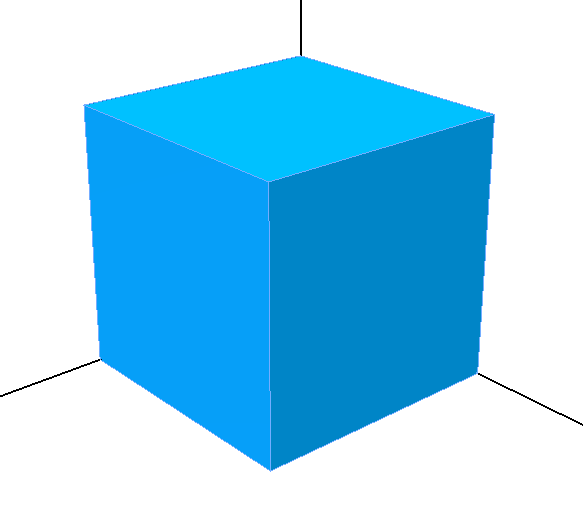
\includegraphics[width=4cm]{cube3Dpos} &
    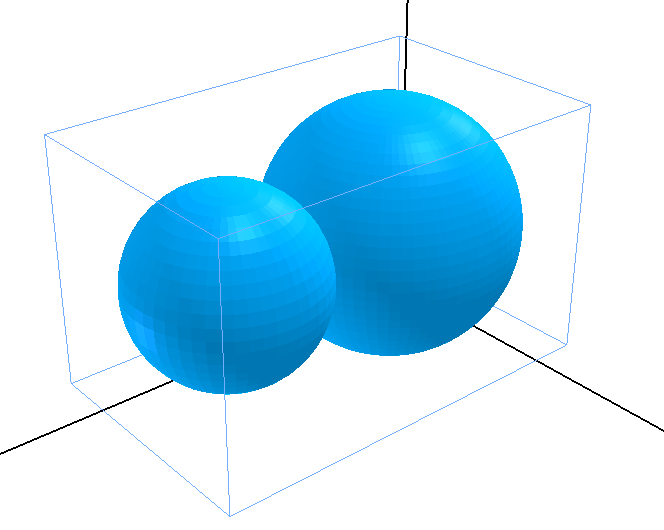
\includegraphics[width=5cm]{vue3D_2spheres}
  \end{tabular}
  \caption{Surfaces dans lesquelles seront effectués les tests}
  \label{fig:envconvdesign}
\end{figure}

\subsubsection{Implémentation}
L'implémentation est définie dans le listing \ref{lst:matcompo}. Il suffit d'insérer l'équation correspondant à nos objets géométriques, ici nos deux sphères. L'équation d'une sphère de centre $M(a,b,c)$ et de rayon $R$ s'écrit $(x-a)^2 + (y-b)^2 + (z-c)^2= R^2$. 
Nommons A l'équation de notre sphère A et B l'équation de notre sphère B, les coordonnées réelles ne nous intéressent que peu ici, nous nous en abstrairons donc. L'opération de différence n'étant pas disponible, il faut la réaliser avec une combinaison d'opérations disponibles. Donc pour réaliser $A-A \cap B$ par exemple, il faudra utiliser l'équation $(A\ XOR\ B)\ AND\ A$. 

\subsubsection{Résultats}
Le premier test, privé des éventuels conflits avec les surfaces, s'est avéré concluant. En regardant les différentes tranches 2D obtenues à l'aide du slicer de la figure \ref{fig:resultconvcube}, on distingue bien la répartition de la matière dans les deux sphères et l'intersection de ces deux dernières. 
\begin{figure}[htb]
\centering
  \begin{tabular}{@{}ccc@{}}
    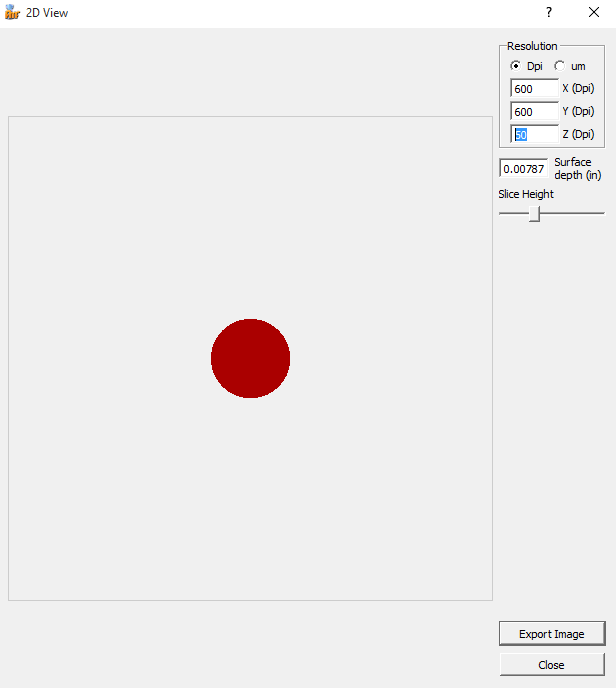
\includegraphics[width=3.7cm]{slice_conv_design_cube_1} &
    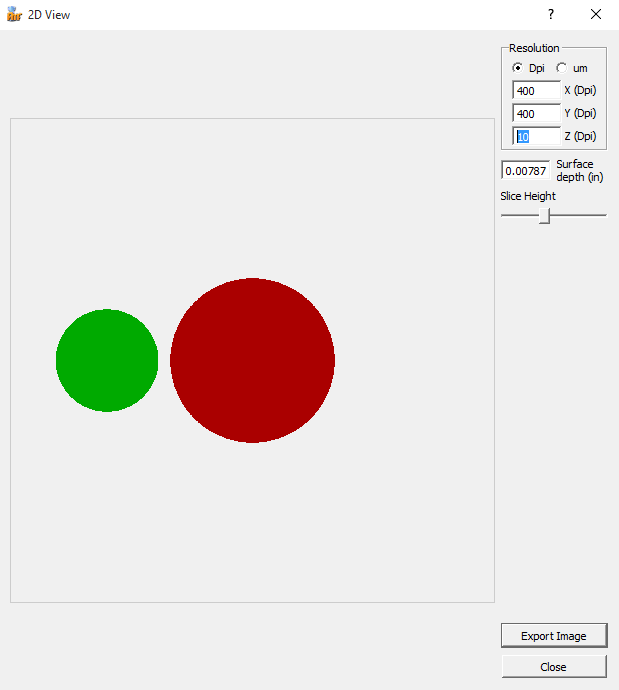
\includegraphics[width=3.7cm]{slice_conv_design_cube_2} &
    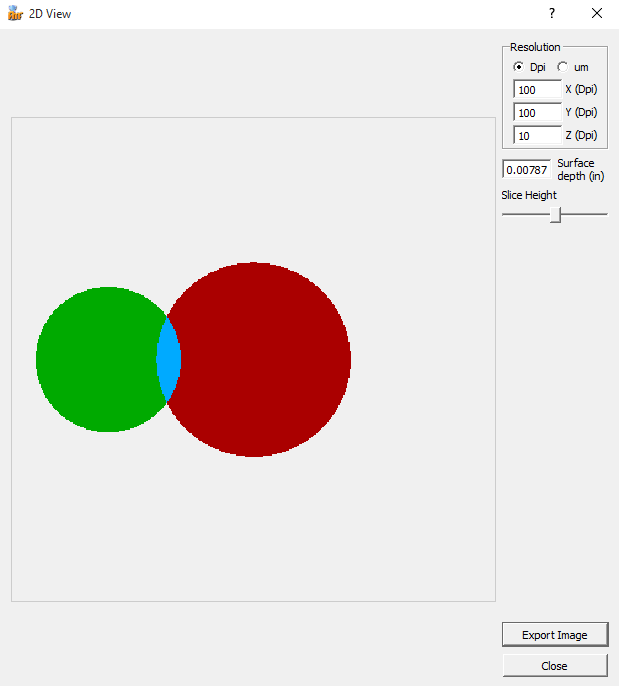
\includegraphics[width=3.7cm]{slice_conv_design_cube_3} \\
    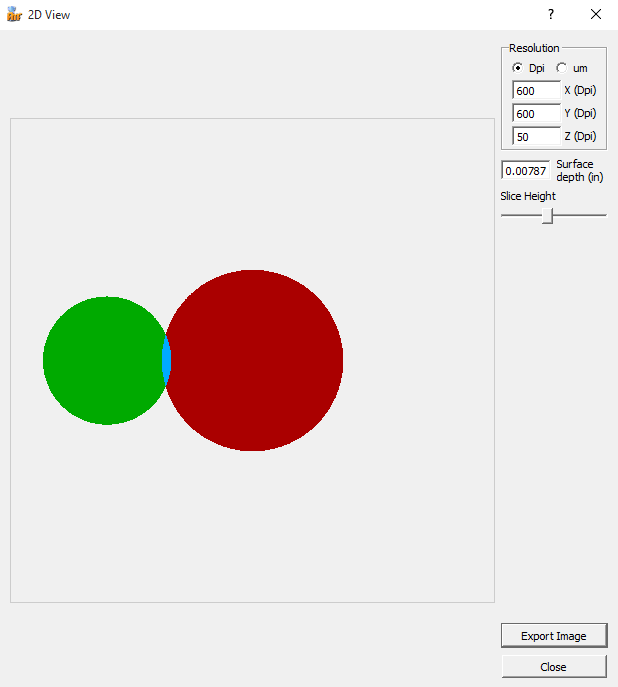
\includegraphics[width=3.7cm]{slice_conv_design_cube_4} &
    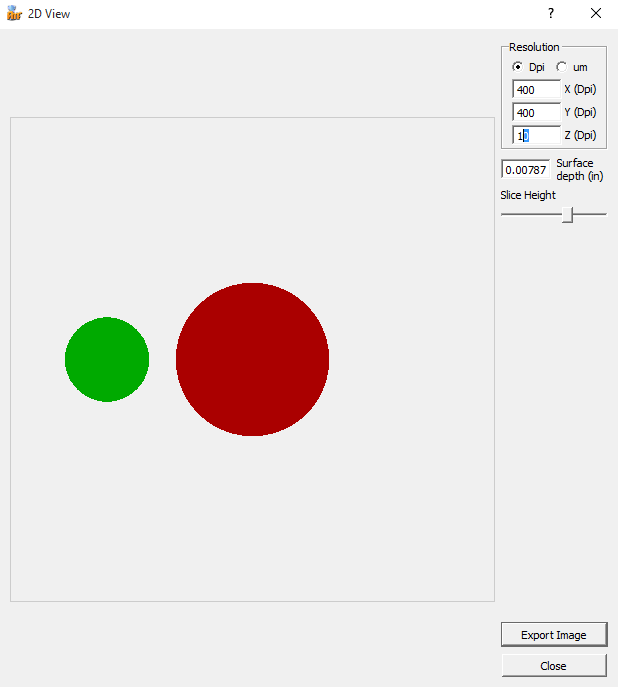
\includegraphics[width=3.7cm]{slice_conv_design_cube_5} &
    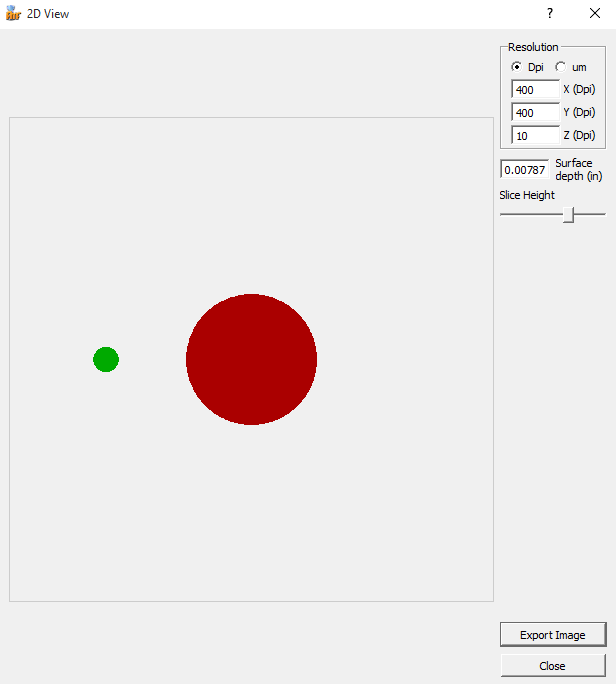
\includegraphics[width=3.7cm]{slice_conv_design_cube_6} 
  \end{tabular}
  \caption{Tranches 2D de bas en haut du cube dans lequel on a défini nos deux sphères}
  \label{fig:resultconvcube}
\end{figure}
Le deuxième test disponible en figure \ref{fig:resultconvspheres} corrobore la possibilité de sauvegarder les intentions de design et plus largement, la structure interne de l'objet via une représentation fonctionnelle. On peut voir ici, contrairement au premier exemple, un fin liseré noir qui représente la surface de l'objet.
\begin{figure}[htb]
\centering
  \begin{tabular}{@{}ccc@{}}
    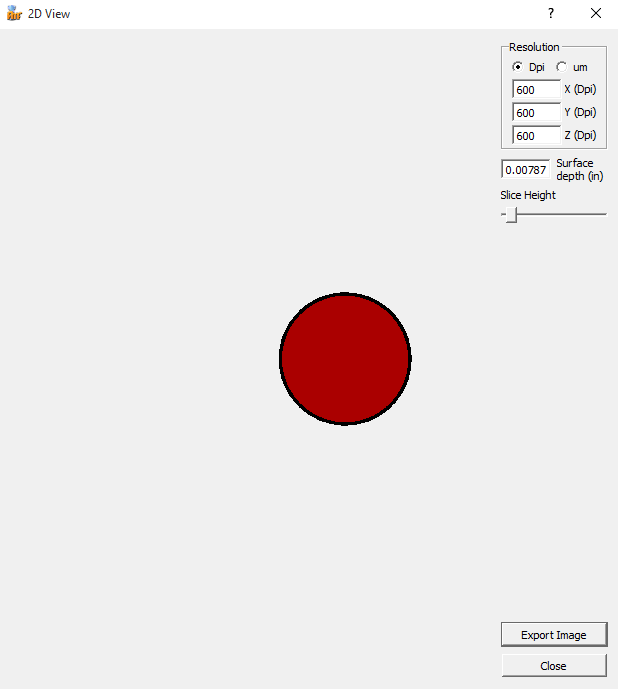
\includegraphics[width=3.7cm]{slice_conserv_design_1} &
    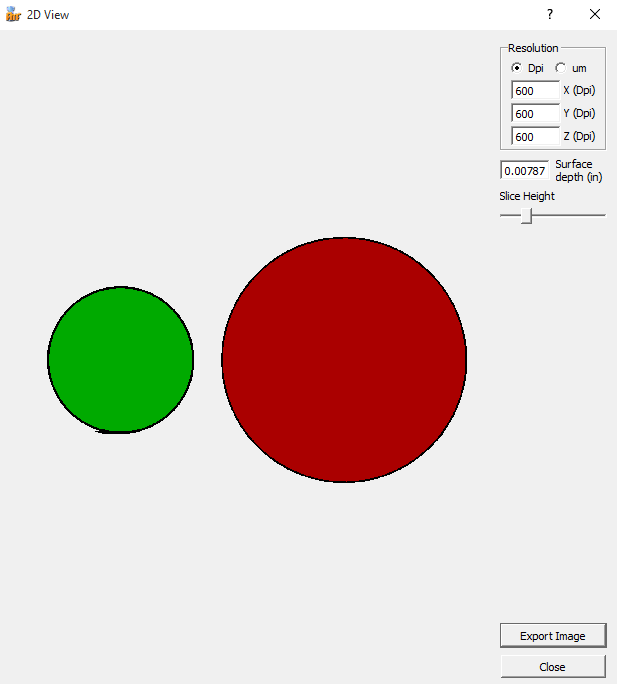
\includegraphics[width=3.7cm]{slice_conserv_design_2} &
    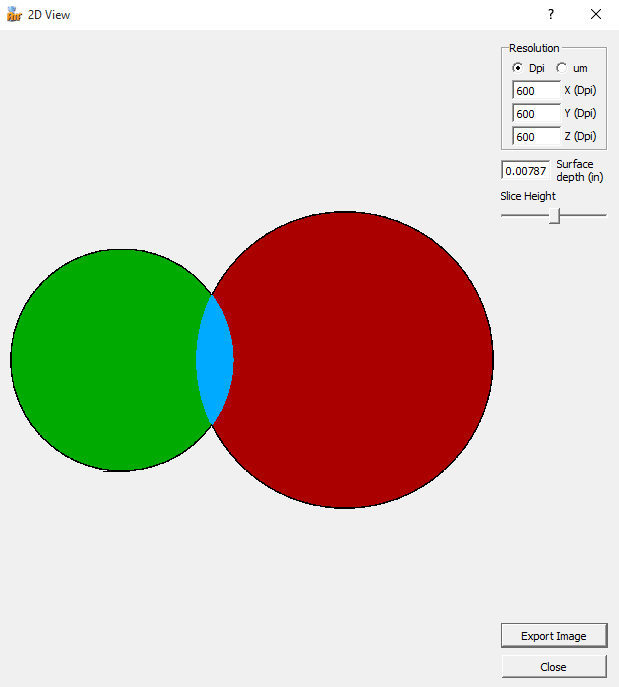
\includegraphics[width=3.7cm]{slice_conserv_design_3} \\
    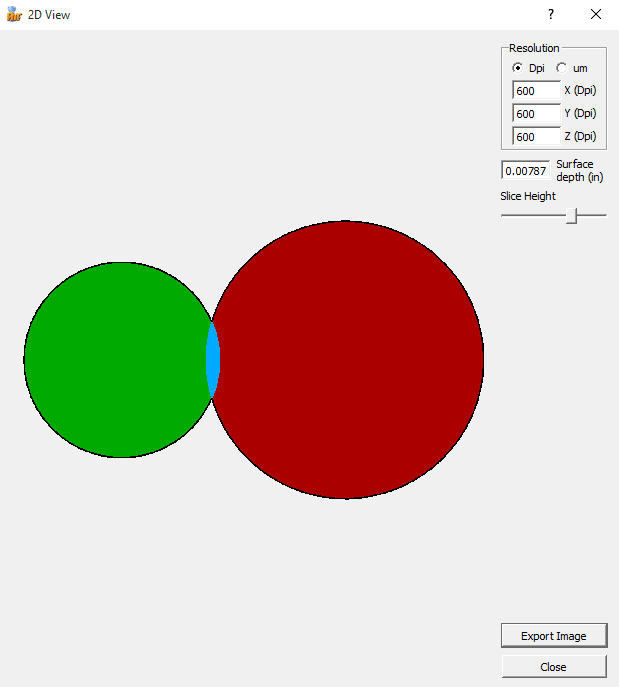
\includegraphics[width=3.7cm]{slice_conserv_design_4} &
    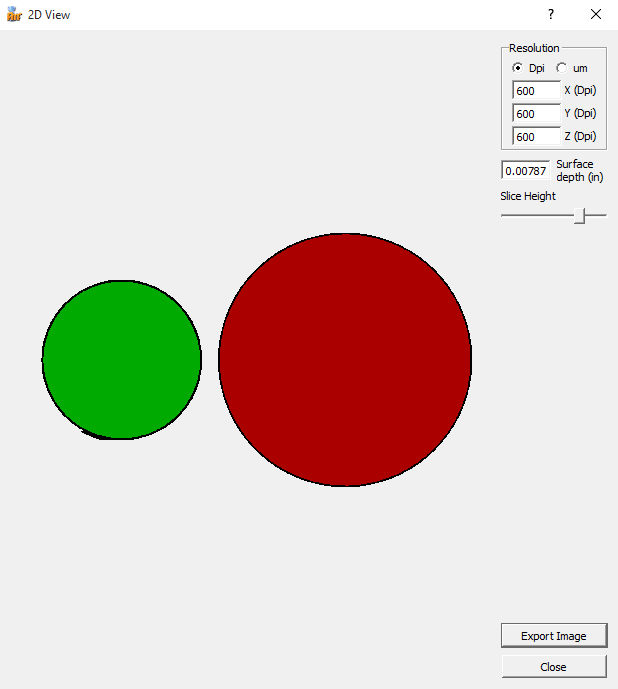
\includegraphics[width=3.7cm]{slice_conserv_design_5} &
    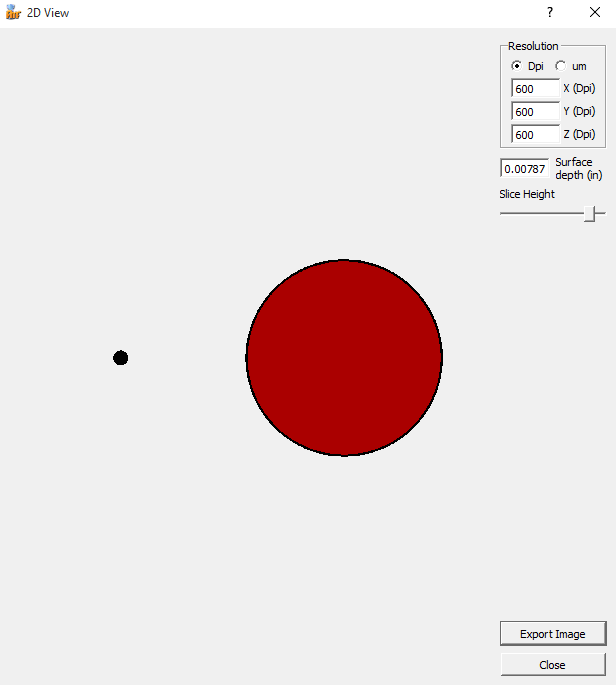
\includegraphics[width=3.7cm]{slice_conserv_design_6} 
  \end{tabular}
  \caption{Tranches 2D de bas en haut des deux sphères}
  \label{fig:resultconvspheres}
\end{figure}
\\
\\
\\
\label{subsec:test2spheres}
Un oeil observateur remarque la redondance des données ici. En effet, si l'on compare les deux tests, il est aisé de se rendre compte que l'on retrouve les même informations. Or, souvenez-vous, lors du premier test, nous avions totalement occulté l'information de surface. Il devient alors évident que toute l'information peut être portée par la définition arithmétique de l'objet, et que l'on peut aisément se passer de la surface polygonale pour définir l'objet. Cela permettrait d'économiser 1.2Mo d'espace (pour un fichier d'1.2Mo, qui ferait alors quelques centaines d'octets), ainsi que de nombreux calculs effectués au niveau du slicing, souvenez-vous de la sous-section \ref{subsec:sliceneff} 



\subsection{Lattices}\label{subsec:lattices}
\subsubsection{Un peu de théorie...}
Une lattice est un ensemble partiellement ordonné d'éléments. En d'autres mots, une lattice définit la répartition des matériaux dans un objet. Étant néophyte dans ce domaine, des recherches supplémentaires ont été nécessaires, afin d'assurer une meilleure compréhension des intérêts et des propriétés de ces lattices. La consultation d'un livre~\cite{latticesbook} sur la théorie des lattices a été très formatrice. Il existe des exemples connus de lattices, notamment dans les théories de pavage\footnote{Remplissage de l'espace selon un schéma défini} de l'espace que l'on peut visualiser sur la figure \ref{fig:lattices_classiques}.
\begin{figure}[h]
  \centering
  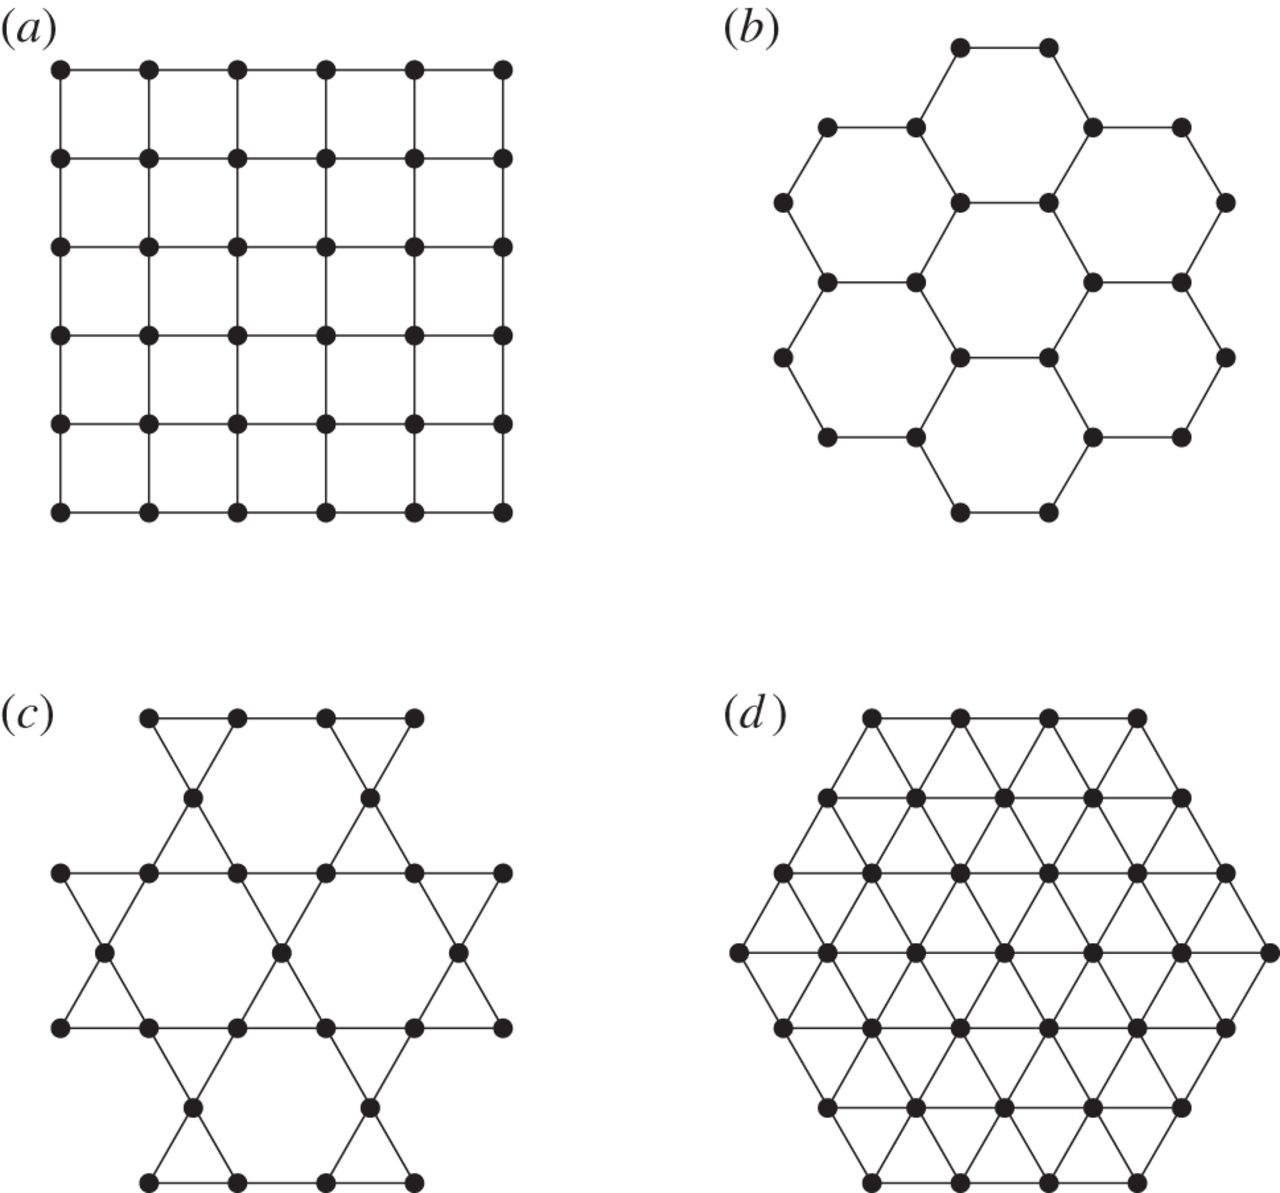
\includegraphics[width=10cm]{lattices_classiques}
  \caption{Exemples de lattices 2D A: carrée, B: nids d'abeille, C: kagomé, B: triangulaire}
  \label{fig:lattices_classiques}
\end{figure}
 Chaque lattice a des caractéristiques propres, la rendant plus adaptée à une application particulière. Prenons la lattice en nids d'abeille en exemple, qui définit le pavage 2D le plus efficace, ce fait ayant été démontré par T. C. Hales dans sa publication nommée "HoneyComb Conjecture"~\cite{hales2001honeycomb}.

Nous pouvons étendre ces considérations d'optimisation en 3D. Le pavage parfait à l'image du nid d'abeille en 2D n'est pas encore connu. Seulement quelques théoriciens se rapprochent de cet idéal à travers leurs propositions, tel Kelvin et son octoèdre tronqué. D'autres chercheurs ont trouvé des pavages semi-réguliers plus efficaces, mais de peu. 

Néanmoins malgré ces considérations, Jérémie Farret indique que selon les technologies d'impression utilisées, de telles théories peuvent devenir non optimales voire problématiques, selon l'orientation des strates de dépôt de matériau, par exemple, ou encore les effets d'aliasing (Crénelage) sur les données d'entrée. Ces perturbations peuvent entraîner une forte variation des caractéristiques essentielles des éléments imprimés, comme leur rigidité . La lattice cubique étant largement utilisée et plus simple à implémenter, elle fera l'objet de nos tests.
\\

Après cette brève description des lattices, on comprend vite l'intérêt de pouvoir stocker ces lattices dans le même fichier que la surface, les deux formant un tout. Cela permet de conserver les propriétés initiales de l'objet, et ainsi le stocker comme il a été conçu. C'est pour cette raison qu'il était important de déterminer dans quelle mesure les lattices étaient supportées, et comment les utiliser. 
\newpage
\subsubsection{Environnement de test}
Il était important de tester l'implémentation des lattices dans de nombreuses configurations d'objets, dans le but d'identifier des erreurs éventuelles. Ces erreurs peuvent être dues à un objet creux ou concave par exemple. Il était également important de représenter les origines possibles\footnote{OpenJscad, site web libre de modélisation 3D, mis en avant dans les consignes du stage, propose un export vers AMF particulier, avec un volume par triangle, ne permettant pas de définir la structure interne de l'objet.} des objets. Différents objets feront donc partie de notre batterie de test. 
\begin{itemize}
  \item Un cube défini directement en AMF visible sur la figure \ref{fig:cube3D}
  \begin{figure}[ht]
    \centering
    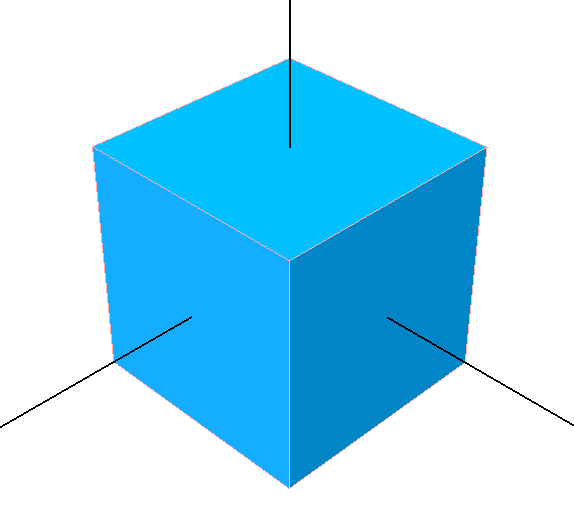
\includegraphics[width=4cm]{cube3D}
    \caption{Vue 3D du cube de test}
    \label{fig:cube3D}
  \end{figure}
  \item Une colonnade réalisée par mes soins sous OpenSCAD\footnote{OpenSCAD, logiciel libre de modélisation 3D, est basé sur la modélisation constructive définie section \ref{sec:csg}} puis exportée vers AMF depuis OpenSCAD. (figure \ref{fig:colonnade3D}).
  \begin{figure}[ht]
    \centering
    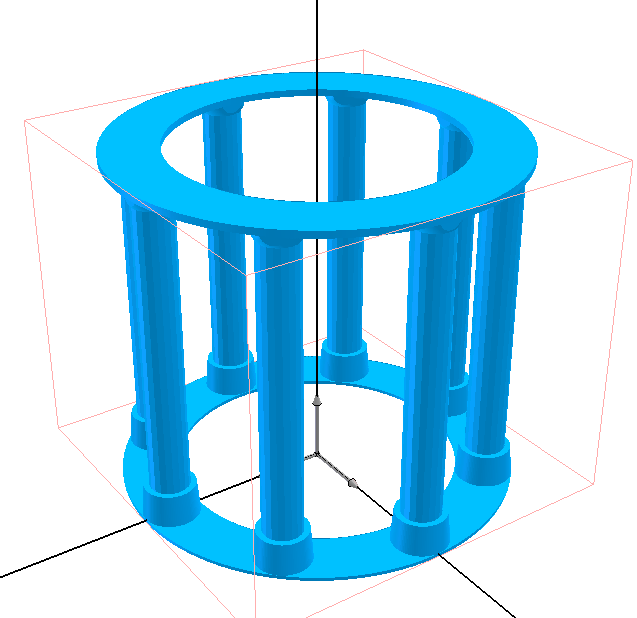
\includegraphics[width=4cm]{colonnade3D}
    \caption{Vue 3D de la colonnade de test}
    \label{fig:colonnade3D}
  \end{figure}
  \item Une réalisation nommée "CircleThing" postée sur ThingInverse\footnote{ThingInverse est un site de partage de fichiers STL lancé par MakerBot}, qui est suffisamment complexe pour effectuer de nombreux tests en un. C'est à l'origine une conception sous OpenSCAD, exportée en fichier STL puis importée en AMF sous AMFTools, elle est illustrée par la figure \ref{fig:circlething3D}.
  \begin{figure}[ht]
    \centering
    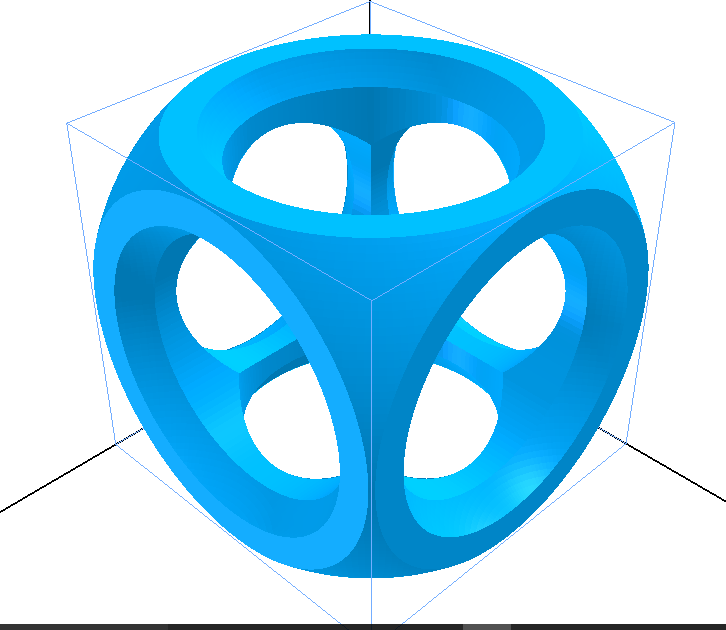
\includegraphics[width=4cm]{circlething3D}
    \caption{Vue 3D de l'objet "circlething" de test}
    \label{fig:circlething3D}
  \end{figure}
\end{itemize}

\subsubsection{Implémentation}

L'implémentation suit celle définie dans le listing \ref{lst:matcompo}. Il suffit d'insérer l'équation correspondant à notre lattice. Il s'avère aisé de définir une lattice cubique grâce à l'opération modulo. Cela donne l'équation suivante : \\
$(mod(abs(x),10)<2) or (mod(abs(y),10)<2) or (mod(abs(z),10)<2)$ \\ 
 Intéressons-nous à la première des trois composantes séparées par un "OU" logique: \\                                $mod(abs(x),10)<2)$. \\
 Simplement, lorsque la valeur absolue de x est proche d'un multiple de 10, cette partie renvoie 1 et partout ailleurs 0. On assignera donc 1 à la "proportion" de matière rouge à cet endroit. Ce qui donne une suite de lignes parallèles, toutes perpendiculaires à l'axe des abscisses. En ajoutant avec un OU logique la même équation, mais cette fois en y, on se retrouve avec un quadrillage donc une lattice carrée. Enfin, en ajoutant z de la même manière, on obtient une lattice cubique.  

\subsubsection{Résultats des tests}

Procédons par étapes, regardons dans un premier temps ce que le test sur le cube a donné. Afin de visualiser le résultat, nous n'avons d'autre choix que de montrer les tranches\footnote{Tranche: coupe en 2D pour une hauteur fixée de l'objet} visualisées à partir du slicer d'AMFTools. Dans le cas du cube illustré en figure \ref{fig:resultlatcube}, on retrouve bien notre lattice cubique, avec sur l'image de gauche la tranche lorsque z n'est pas proche d'un multiple de 10. Et à droite la tranche quand z est proche d'un multiple de 10, formant ainsi une couche de matière uniforme. Le test est donc concluant.
\begin{figure}[htb]
\centering
  \begin{tabular}{@{}cc@{}}
    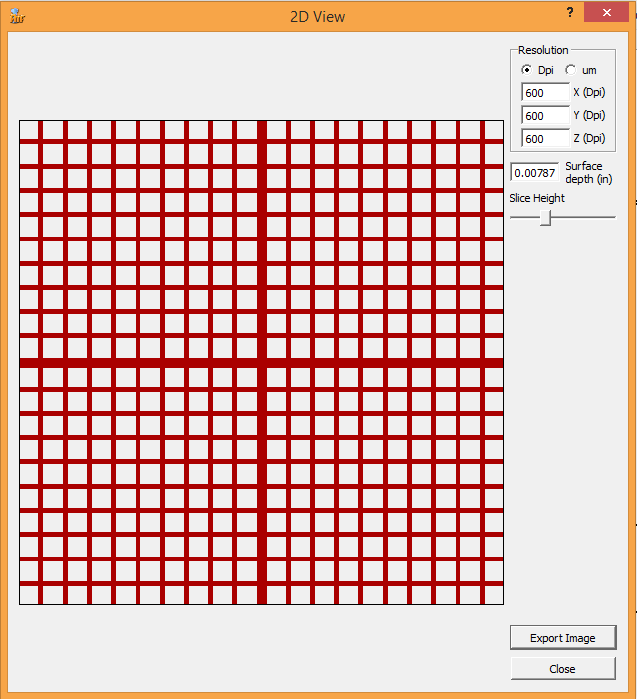
\includegraphics[width=6.5cm]{slice_lattice_cubique_centree} &
    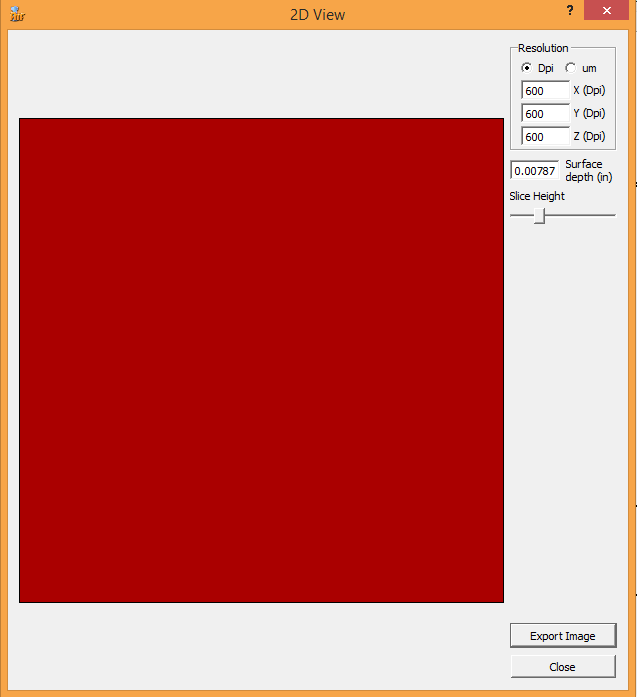
\includegraphics[width=6.5cm]{slice_tranche_lattice_cubique}
  \end{tabular}
  \caption{Tranches 2D du cube rempli avec une lattice cubique}
  \label{fig:resultlatcube}
\end{figure}

Intéressons-nous maintenant au remplissage de notre colonnade tel qu'illustré par la figure \ref{fig:resultlatcol}. La tranche de gauche étant réalisée au niveau des colonnes, tandis que la droite se situe au niveau de l'anneau au sommet des colonnes. une fois de plus, on retrouve notre lattice, correctement définie dans l'objet, le test est également concluant.

\begin{figure}[htb]
\centering
  \begin{tabular}{@{}cc@{}}
    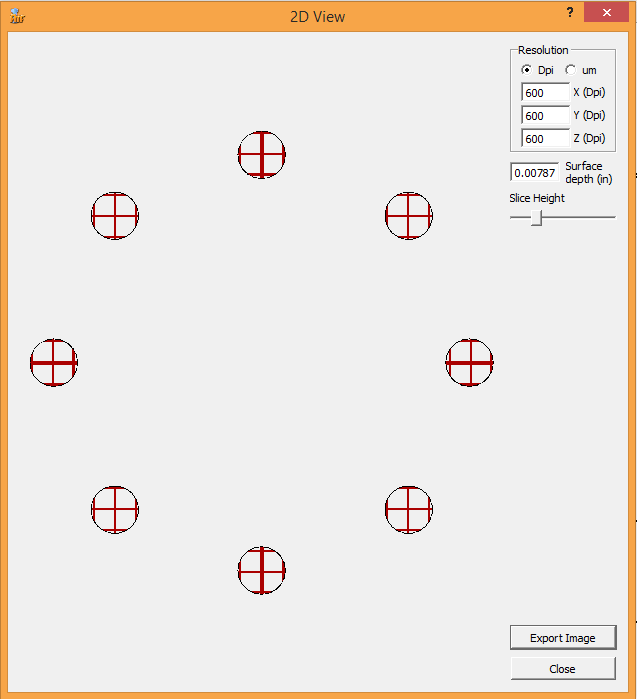
\includegraphics[width=6.5cm]{slice_lattice_cubique_dans_colonnade} &
    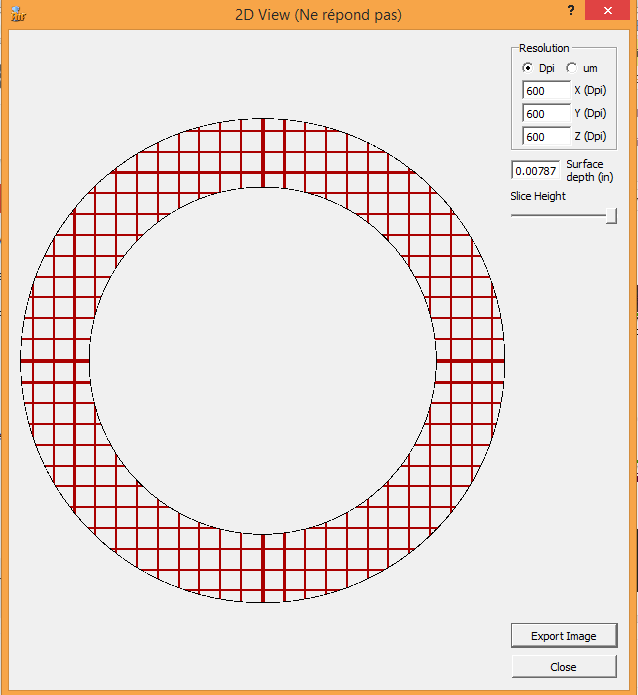
\includegraphics[width=6.5cm]{slice_lattice_cubique_dans_colonnade_anneau}
  \end{tabular}
  \caption{Tranches 2D de la colonnade remplie avec une lattice cubique}
  \label{fig:resultlatcol}
\end{figure}

\newpage
Dernier élément, certainement l'exemple le plus significatif, notre "circlething". On peut parfois voir des bavures, engendrées par le slicer, mais elles paraissent aléatoires. Malgré ce défaut du slicer, les résultats obtenus, illustrés par la figure \ref{fig:resultlatcircle}, confirment les résultats précédents et permettent d'affirmer que les lattices sont bel et bien utilisables dans la version actuelle du couple AMF/AMFTools.

\begin{figure}[htb]
\centering
  \begin{tabular}{@{}cc@{}}
    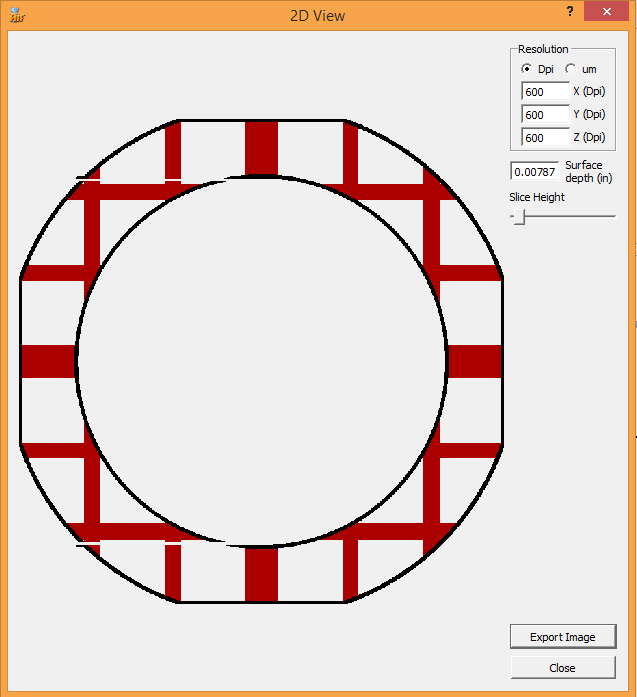
\includegraphics[width=4.6cm]{slice_circle_thing_2} &
    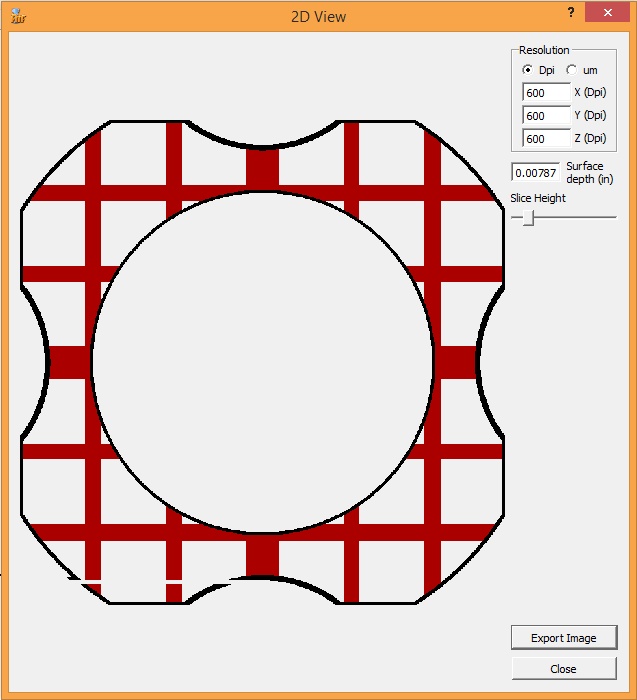
\includegraphics[width=4.6cm]{slice_circle_thing_3} \\
    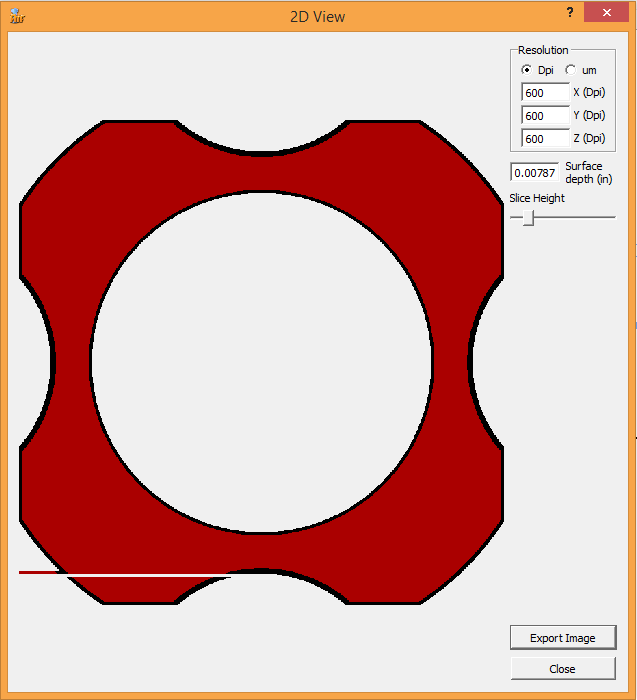
\includegraphics[width=4.6cm]{slice_circle_thing_4} &
    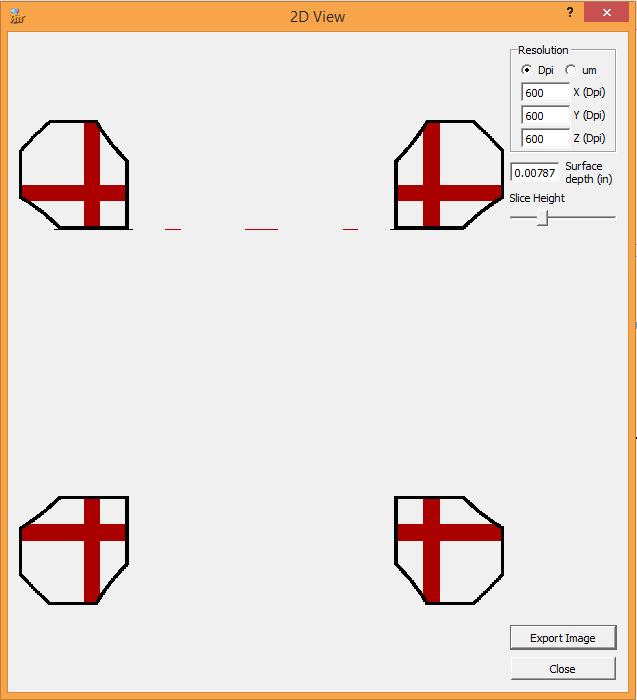
\includegraphics[width=4.6cm]{slice_circle_thing_6}
  \end{tabular}
  \caption{Tranches 2D de "circlething" remplie avec une lattice cubique}
  \label{fig:resultlatcircle}
\end{figure}

\newpage
\subsection{Représentation de données voxel en AMF}
\label{subsec:repvoxel}
L'utilisation de voxels\footnote{Un voxel est un pixel en 3D, on lui attribue une position dans l'espace, ainsi qu'un nombre non borné de propriétés} explosant ces dernières années, il est intéressant pour une norme comme AMF d'être capable de l'intégrer. Certains acteurs du workgroup AMF utilisent des données voxels dans leurs domaines respectifs, plus particulièrement dans le domaine de la santé, pour de nombreux type d'imagerie médicale, tel la tomographie\footnote{technique de numérisation de données non intrusives, consistant en la mesure tranche par tranche, avant de reconstruire l'objet analysé en empilant ces tranches}. Deux approches ont été dégagées pour stocker des données voxels en AMF. La première, émise par le Workgroup AMF, consiste à créer un volume pour chaque voxel. La seconde, imaginée à partir des travaux déjà réalisés au sein du stage, consiste en l'export de la surface de l'objet en voxels et le stockage des voxels internes via la représentation fonctionnelle.

\subsubsection{Approche Multi-volumes}
 Il s'agit ici d'exploiter l'outil constellation proposé par AMF. Le concept est simple, il suffit de définir nos différents objets dans un premier temps. Dans notre cas, nous n'aurons que des cubes 1x1x1, mais il faut en définir un pour chaque matière différente que l'on souhaite représenter. Par la suite on définit une constellation\footnote{Les identifiants sont partagés avec les éléments d'autres types, il convient donc d'assigner un id unique à cette dernière.} comme l'illustre le listing \ref{lst:constel}, en créant des instances de chaque objet, copie conforme de l'objet défini, mais en précisant sa position ainsi que sa rotation dans l'espace.
 
\begin{lstlisting}[language=AMF,label={lst:constel},caption={syntaxe d'utilisation d'une constellation}]
  <constellation id="3">
    <metadata type="name">Constellation principale</metadata>
    <instance objectid="1">
      <deltax>0</deltax>
      <deltay>0</deltay>
      <deltaz>0</deltaz>
      <rx>0</rx>
      <ry>0</ry>
      <rz>0</rz>
    </instance>
    <instance objectid="2">
      <deltax>2</deltax>
      <deltay>0</deltay>
      <deltaz>0</deltaz>
      <rx>0</rx>
      <ry>0</ry>
      <rz>0</rz>
    </instance>
  </constellation>
\end{lstlisting}

Il est également possible d'affecter une texture à la surface de notre cube, ce qui a été réalisé dans le cadre de l'exemple, mais cette partie est suffisamment documentée dans la norme\cite{astmAMF} et ne sera pas traitée dans ce rapport. Le logo d'AMF étant une tour, c'est cette forme qui a été choisie dans le cadre de notre test dont le résultat est visible sur la figure \ref{fig:tourvox}
\begin{figure}[h]
  \centering
  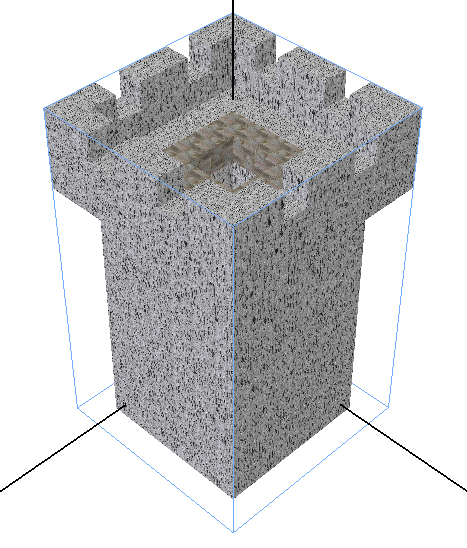
\includegraphics[width=6cm]{tour3D}
  \caption{Vue 3D de la tour voxel}
  \label{fig:tourvox}
\end{figure}

D'après la vue 3D, il pourrait tout à fait s'agir d'un seul objet. La vue en tranches de la figure \ref{fig:slicetourvox} permet néanmoins de visualiser sa structure.
\begin{figure}[htb]
\centering
  \begin{tabular}{@{}ccc@{}}
    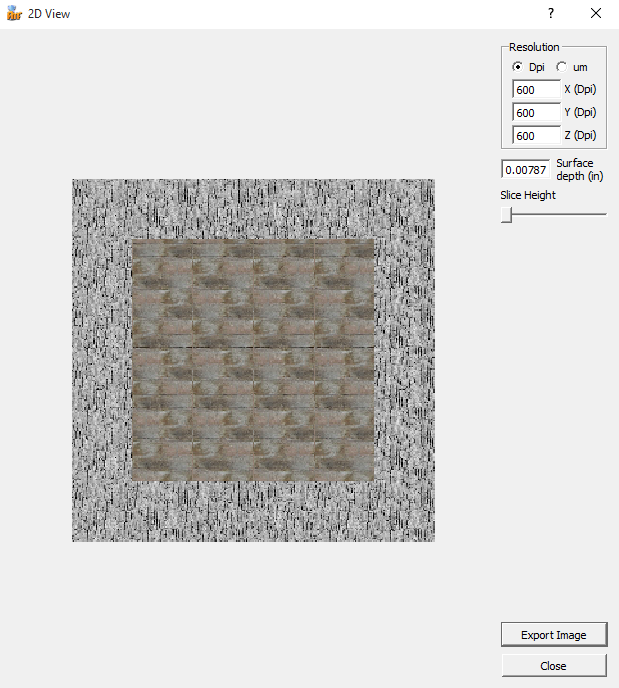
\includegraphics[width=4cm]{slice_tour_1} &
    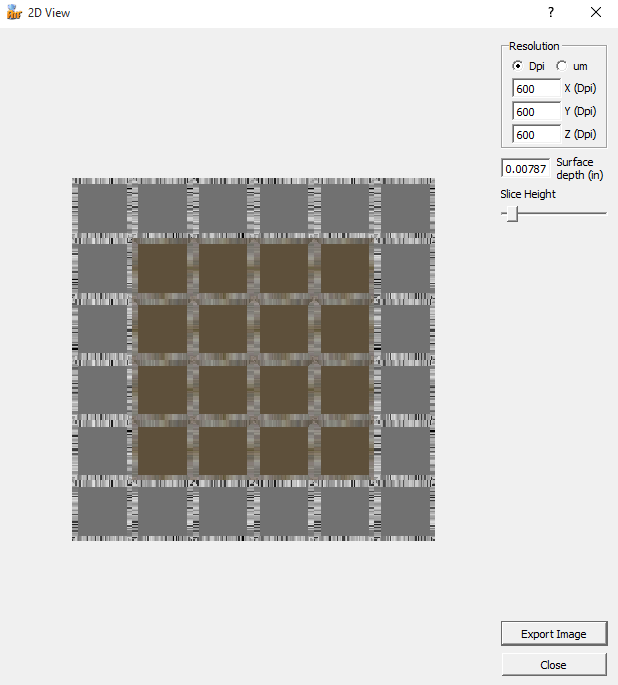
\includegraphics[width=4cm]{slice_tour_2} &
    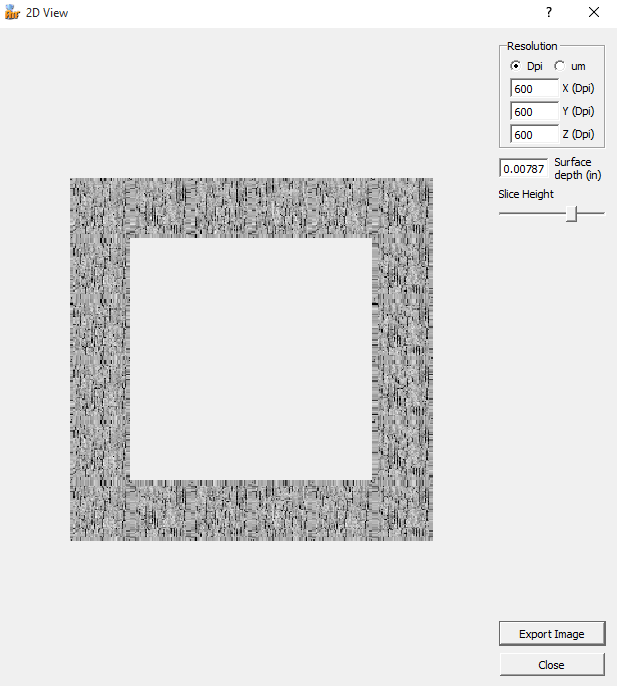
\includegraphics[width=4cm]{slice_tour_3} \\
    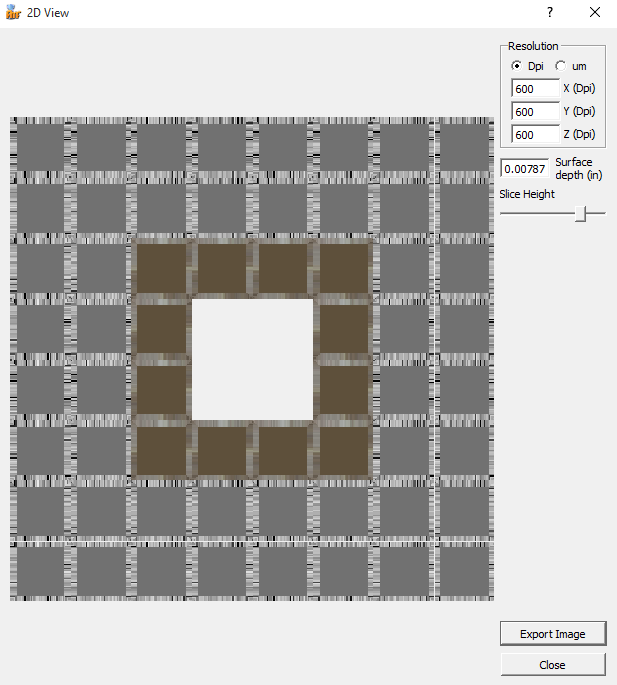
\includegraphics[width=4cm]{slice_tour_4} &
    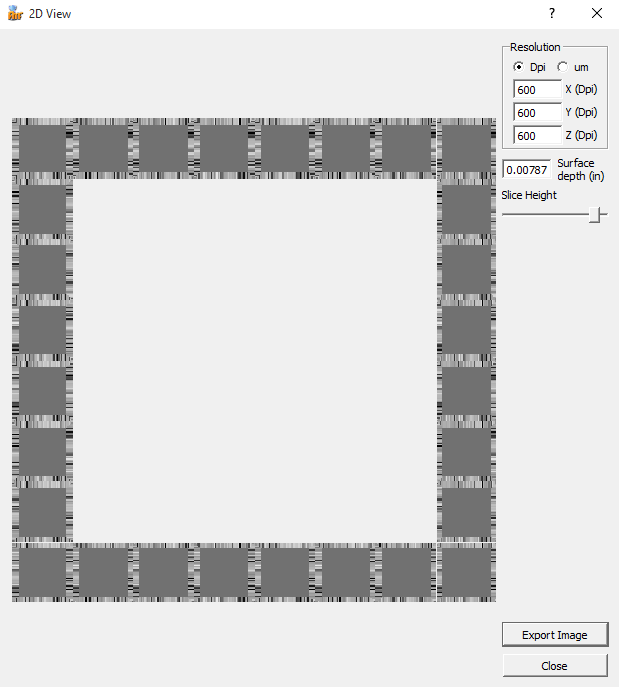
\includegraphics[width=4cm]{slice_tour_5} &
    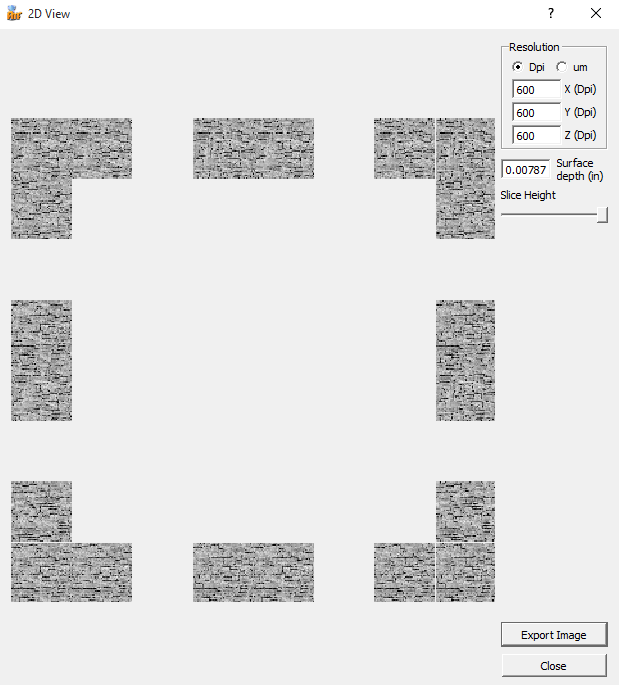
\includegraphics[width=4cm]{slice_tour_6} \\
  \end{tabular}
  \caption{Tranches de bas en haut de la tour voxel}
  \label{fig:slicetourvox}
\end{figure}

Ces tests prouvent donc qu'il est possible de stocker des données voxels dans le format AMF, sans perte de données. Cela s'accompagne des caractéristiques des données voxels, particulièrement leur volume. Plus l'objet est grand et plus la précision est grande - plus les voxels sont petits - plus la taille mémoire de l'objet va augmenter. On peut facilement se retrouver avec des fichiers de tailles vraiment conséquentes. Il existe une optimisation classique, consistant à ranger nos pixels sous formes d'octree\footnote{optimisation de l'espace permettant parfois de réduire drastiquement le nombre de voxels nécessaires à la représentation de l'objet.}. On construit un arbre qui subdivise chaque cube en 8 s'il contient des variations. En commençant par un cube contenant tous les voxels, en subdivisant afin de ne perdre aucun détail. En d'autres termes, si huit cubes identiques forment un cube, on stockera uniquement ce cube. Il est possible de représenter des données voxels optimisées par Octree, mais paradoxalement, même si cela réduit le nombre de voxels enregistrés, cela nécessite la définition d'autant de meshs que de niveaux de subdivision de l'octree. Ce qui peut représenter de nombreux octets.   

\subsubsection{Approche fonctionnelle}
L'idée est d'exploiter la représentation fonctionnelle précédemment démontrée afin de modéliser les voxels à l'intérieur de la surface polygonisée de l'objet voxel.
Afin de faciliter la génération d'un exemple convaincant, l'outil en ligne proposé par 3DSlash\cite{3DSlash} a été utilisé. Cet outil permet de réaliser facilement un objet en ajoutant/enlevant des voxels à une cuve de voxels. La figure \ref{fig:voxels3D} permet de visualiser l'objet de test. Il est possible également d'appliquer une texture à cette surface pour correspondre au rendu des voxels internes, mais cela sort du cadre de notre test. 
\begin{figure}[h]
  \centering
  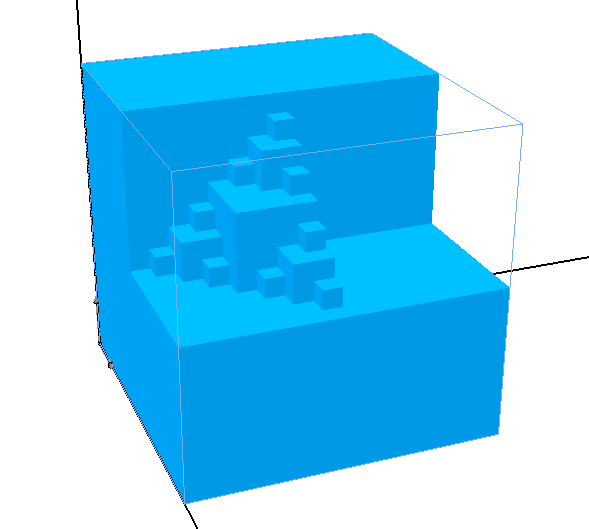
\includegraphics[width=6cm]{voxels3D}
  \caption{Vue 3D de la surface de test}
  \label{fig:voxels3D}
\end{figure}

La définition fonctionnelle de chaque voxel est simple, il est délimité par 6 plans, coïncidents avec ses faces. Ce qui donne concrètement comme équation :\\
\\
$x>Xmin\quad AND\ x<Xmax\ AND\ y>Ymin\ AND\ y<Ymax\ AND\ z>Zmin\ AND\ z<Zmax$ \\
\\
Pour l'implémenter, il suffit de placer cette équation dans l'emplacement prévu à cet effet dans le listing \ref{lst:matcompo} et d'assigner la matière désirée en choisissant le materialid correspondant. C'est simple et cela permet de représenter des données voxels optimisées par octree sans coût de volume de fichier supplémentaire. 

Le résultat du test sur la figure \ref{fig:slicevoxels} met bien en avant la possibilité d'optimisation par octree via les voxels de différentes tailles.  
\begin{figure}[htb]
\centering
  \begin{tabular}{@{}cc@{}}
    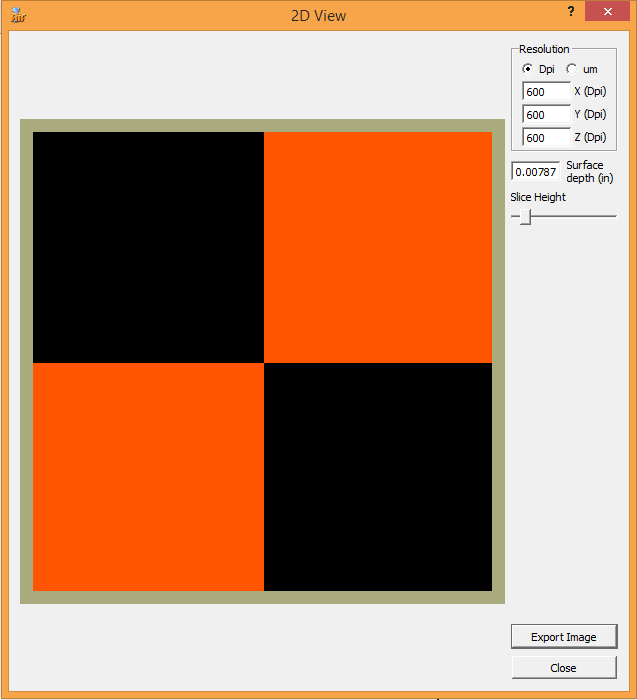
\includegraphics[width=5cm]{slice_cubes_voxels_1} &
    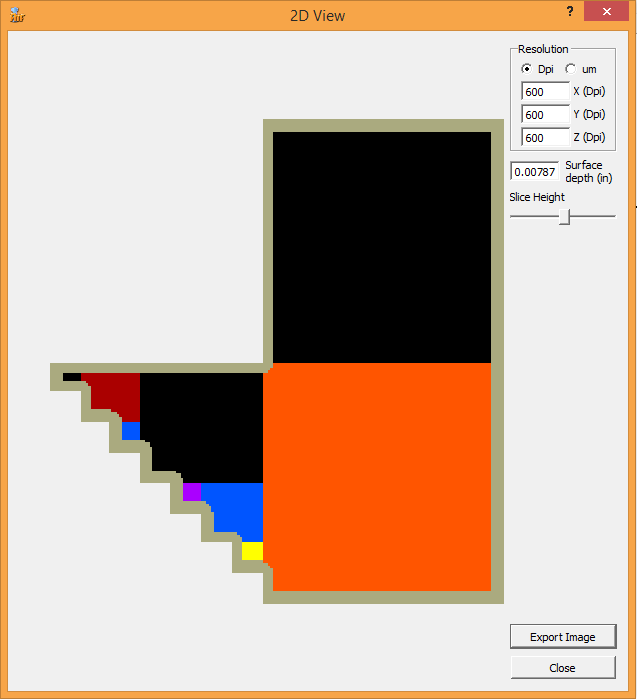
\includegraphics[width=5cm]{slice_cubes_voxels_2} \\
    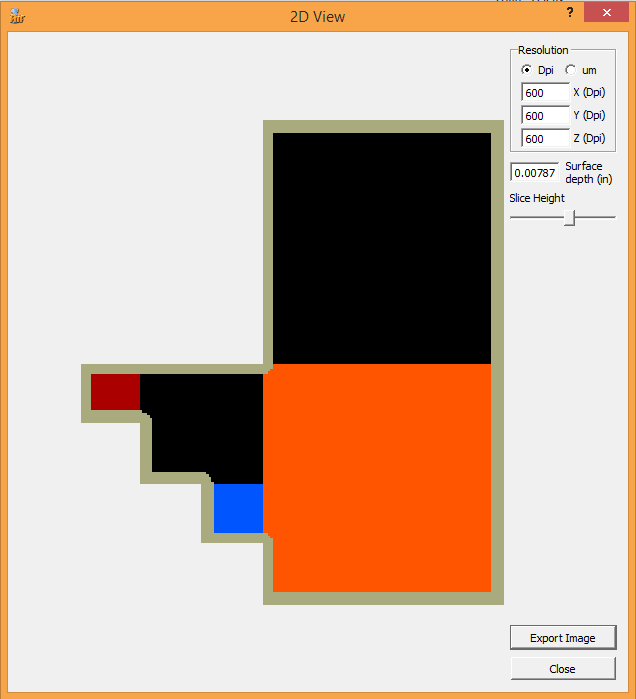
\includegraphics[width=5cm]{slice_cubes_voxels_3} &
    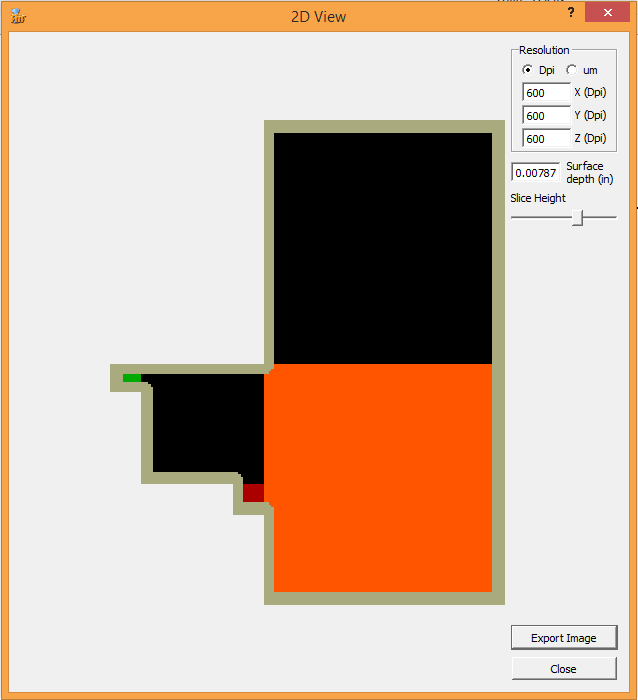
\includegraphics[width=5cm]{slice_cubes_voxels_4} \\
    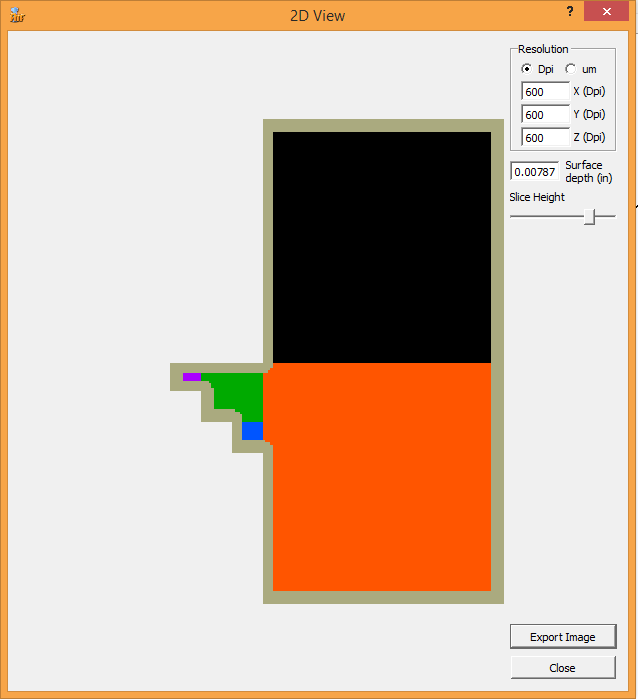
\includegraphics[width=5cm]{slice_cubes_voxels_5} &
    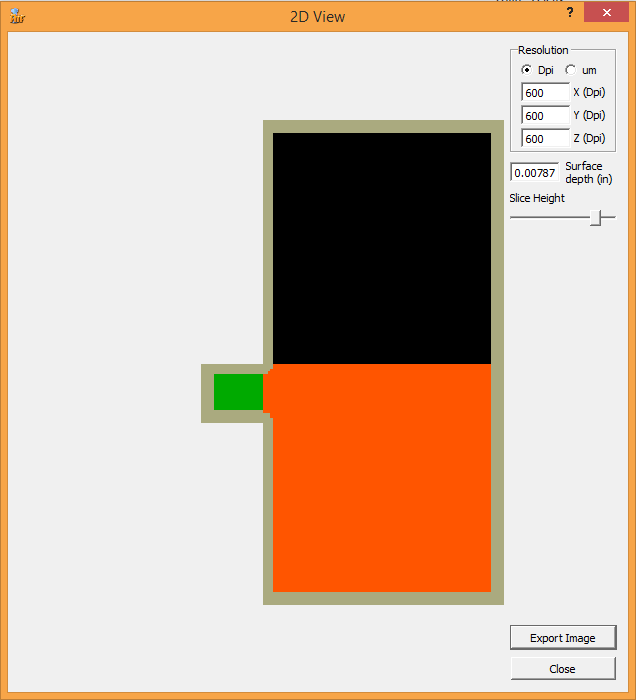
\includegraphics[width=5cm]{slice_cubes_voxels_6} \\
    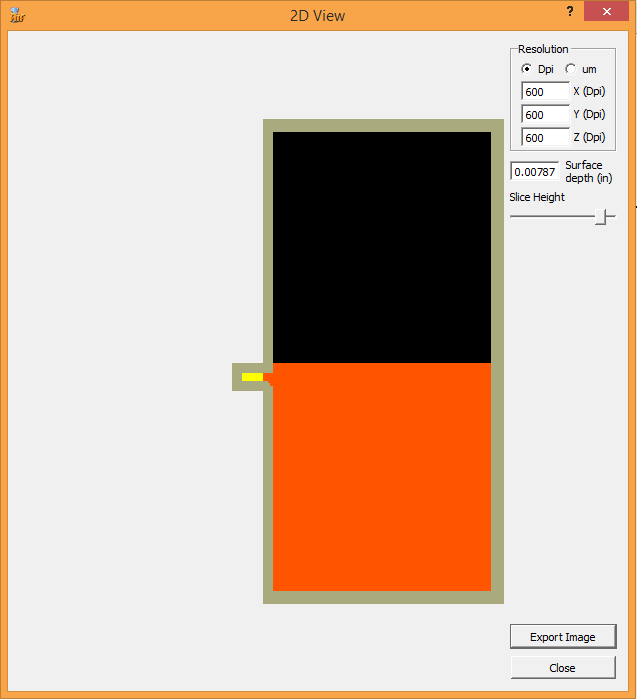
\includegraphics[width=5cm]{slice_cubes_voxels_7} &
    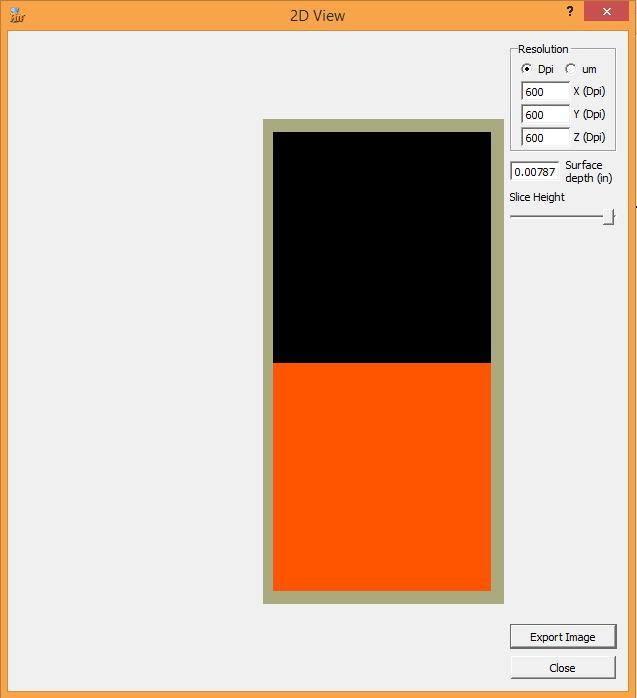
\includegraphics[width=5cm]{slice_cubes_voxels_8} \\
  \end{tabular}
  \caption{Tranches de bas en haut de notre objet}
  \label{fig:slicevoxels}
\end{figure}
Cette approche comporte une certaine limitation, se situant dans le temps de calcul nécessaire au slicer. En effet, comme vu précédemment, le slicer étant de type voxel, la complexité du calcul final peut poser problème lors du traitement de grandes instances. 

\clearpage
\subsection{Texturing 3D}
\label{subsec:tex3D}
L'application d'une texture sur la surface externe est connue et documentée, elle ne fait donc pas l'objet de ce stage. En revanche l'utilisation de texture 2D et 3D pour définir la structure interne de l'objet nous intéresse tout particulièrement. L'intégration d'une image dans un fichier AMF a été traité dans la sous-section \ref{subsec:conv}, nous n'y reviendrons donc pas. L'objectif est ici de stocker l'information de répartition de la matière dans une texture et d'arriver à utiliser cette information. 

\subsubsection{Environnement de test}

Il est possible d'effectuer ce test dans n'importe quelle forme de surface, mais dans un premier temps, dans le but de simplifier l'expérience, nous nous limiterons à des cubes de différentes tailles. Coté textures, notre ensemble de tests visible en figure \ref{fig:textures} a été converti en textures AMF selon la méthode décrite dans la sous-section \ref{subsec:conv}. L'idée de ce panel est de tester toutes les textures sur des cubes de différentes tailles, afin de voir de quelle manière AMFTools réagirait. Les cubes sont de tailles 1*1*1,2*2*2,10*10*10,32*32*32,100*100*100 et ont été générés à partir du cube 1*1*1 déjà utilisé dans d'autres tests dont le visuel est disponible sur la figure \ref{fig:cube3D}. Ici l'unité définie est le mm. Après validation des tests avec des textures 2D, des tests utilisant des textures 3D seront mis en place.
\begin{figure}[htb]
\centering
  \begin{tabular}{@{}ccccc@{}}
    
\includegraphics[width=2cm]{pixel_vert_1} &
    
\includegraphics[width=2cm]{4pixels_50} &
    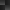
\includegraphics[width=2cm]{carreaux_10} &
    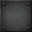
\includegraphics[width=2cm]{plaque_metal_32} &
    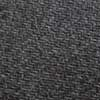
\includegraphics[width=2cm]{tissu_100} 
  \end{tabular}
  \caption{Textures de test}
  \label{fig:textures}
\end{figure}

\subsubsection{Implémentation}
\label{subsec:imptext}
On utilise toujours ici la représentation fonctionnelle pour définir la structure interne de notre objet, définie dans la section \ref{subsec:mathdesc}. On s'intéressera ici plus particulièrement à la fonction tex(texid,u,v,w) disponible dans AMF. Cette fonction, d'après sa description dans la lettre d'ouverture d'AMF\cite{articlebaseAMF}, renvoie une valeur entre 0 et 1 correspondant au pixel de coordonnées u, v et w. Après quelques tests préliminaires, il a été déterminé que l'indexation des textures allait de $0$ à $NombrePixels-1$. Les coordonnées u, v, et w que l'on doit fournir sont des entiers. Comme le montre la section \ref{subsec:etuslicer}, le slicer ne prenant pas en compte les éléments internes proches de la surface, il n'est pas nécessaire de se prémunir contre un dépassement en enlevant la valeur maximale. Dans ce cadre, pour obtenir u en fonction de x, tout en prenant en compte la taille de la texture ainsi que celle de l'objet à texturer, on obtient la formule suivante : $u=floor(x*\frac{Nombre\_de\_pixels}{Taille\_objet})$ \\ Ce qui donne pour l'équation de répartition de la matière : \\ $tex(1,floor(x*\frac{Nombre\_de\_pixels}{Taille\_objet}),floor(y*\frac{Nombre\_de\_pixels}{Taille\_objet}))$ \\
Remarquez ici que l'id de la texture est 1, ce qui correspond dans notre exemple à la texture en niveaux de gris représentant le rouge. Il convient donc d'assigner un matériau rouge à cette équation.

Si l'on prend par exemple une texture 10*10 et un cube 2*2*2 cela donne le code AMF du listing \ref{lst:equatex}, les textures 1, 2 et 3 correspondant respectivement aux niveaux de rouge, vert et bleu. 
\begin{lstlisting}[language=AMF, caption={Implémentation de la texture dans le solide}, label={lst:equatex}]
  <material id="1">
    <metadata type="name">R</metadata>
    <color>
      <r>1</r>
      <g>0</g>
      <b>0</b>
    </color>
  </material>
  <material id="2">
    <metadata type="name">G</metadata>
    <color>
      <r>0</r>
      <g>1</g>
      <b>0</b>
    </color>
  </material>
  <material id="3">
    <metadata type="name">B</metadata>
    <color>
      <r>0</r>
      <g>0</g>
      <b>1</b>
    </color>
  </material>
  <material id="4">
    <metadata type="name">Texture</metadata>
    <color>
      <r>0</r>
      <g>0</g>
      <b>0</b>
    </color>
    <composite materialid="1"><![CDATA[tex(1,floor(x*10/2),floor(y*10/2))]]></composite>
    <composite materialid="2"><![CDATA[tex(2,floor(x*10/2),floor(y*10/2))]]></composite>
    <composite materialid="3"><![CDATA[tex(3,floor(x*10/2),floor(y*10/2))]]></composite>
</material>
\end{lstlisting}

\subsubsection{Résultats des tests}
L'application de chaque texture à chaque cube a été effectuée dans le cadre de ces tests. Nous ne présenterons en revanche ici qu'un condensé des visuels obtenus, en éliminant les informations redondantes, ne conservant ainsi que les éléments significatifs. 
La première série de tests s'est effectuée sur la texture 1*1, que l'on nommera ici texture 1. Les cubes seront également référencés par leur côté, par exemple cube 10 pour un cube de 10*10*10. 
\begin{figure}[htb]
\centering
  \begin{tabular}{@{}cccc@{}}
    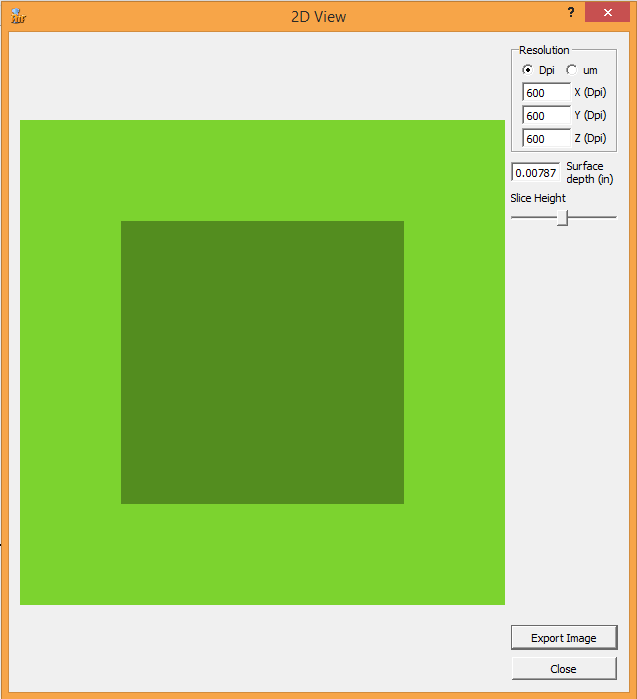
\includegraphics[width=4cm]{slice_cube_1_texture_1pixel_changement_couleur} &
    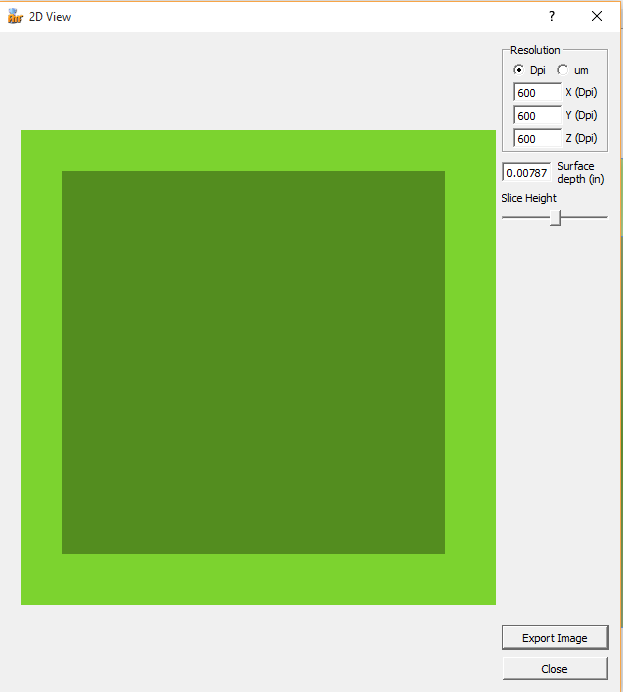
\includegraphics[width=4cm]{slice_cube_2_texture_1pixel_middle} &
    \includegraphics[width=4cm]{slice_cube10_texture1} &
    \includegraphics[width=4cm]{slice_cube_256_texture_1pixel_1_middle}
  \end{tabular}
  \caption{Application de la texture 1 aux cubes 1,2,10,256}
  \label{fig:slicestex1}
\end{figure}
La figure \ref{fig:slicestex1} montre les tranches obtenues lors de ce permier test. On peut voir que dans le cas des cubes 1 et 2, auxquels on applique la texture 1, cela fonctionne, à un écart de couleur près, explicité lors de l'étude du slicer dans la sous-section \ref{subsec:etuslicer}. Mais si l'on se penche sur les deux résultats de droite, on pourrait croire à un nouvel écart de couleur, mais si c'était le cas la couleur serait plus fade en raison des modifications volontaires appliquées par le slicer. Il s'agit donc ici d'une erreur du slicer. \\



Prenons maintenant le cube 1 et appliquons-lui différentes textures. Le résultat obtenu, disponible en figure \ref{fig:slicescube1}, montre un résultat positif dans le cas de la texture 2, mais des résultats totalement incohérents pour les textures 10 et 32. On semble ici avoir affaire à des erreurs d'accès mémoire. La fonction tex() n'est donc pas fonctionnelle en l'état.
\begin{figure}[htb]
\centering
  \begin{tabular}{@{}ccc@{}}
    \includegraphics[width=4cm]{slice_cube_1_texture_4_pixels_middle} &
    \includegraphics[width=4cm]{slice_cube_1_texture_carreaux_10_middle} &
    \includegraphics[width=4cm]{slice_cube_1_texture_plaque_metal_32_middle}
  \end{tabular}
  \caption{Application des textures 2, 10 et 32 au cube 1}
  \label{fig:slicescube1}
\end{figure}

Suite aux résultats de ces tests, et la correction de bugs ne faisant pas partie des objectifs du stage, il a été décidé d'envoyer un rapport d'erreur au groupe de travail AMF. Ce rapport d'erreur a été réalisé par Jérémie Farret, sur la base des travaux de ce stage.

\subsection{Support polygonal de sources solides}\label{subsec:suppoly}
L'objectif de cette section est d'identifier la capacité d'AMF à contenir des conceptions solides initialement réalisées en CSG ou en arithmétique des formes. Cela concerne plus précisément des fichiers complexes, composés de plusieurs volumes ayant des propriétés propres. Il est donc question d'analyser le comportement d'AMF lorsque des objets sont ajustés avec précision, avec par exemple des surfaces en contact. 

\subsubsection{Environnement de test}
L'objet servant de base à nos test est la vasque Frank Lloyd Wright\footnote{Frank Lloyd Wright est un célèbre architecte américain}, modélisée en arithmétique des formes. On peut la voir ainsi que ses éléments constitutifs sur la figure \ref{fig:urnevia}. Afin de simplifier l'exemple, seuls deux éléments différents seronts exportés vers AMF, d'un coté le plateau, coloré en rouge, et de l'autre le reste de la vasque d'un seul bloc.  
\begin{figure}[htb]
\centering
  \begin{tabular}{@{}cc@{}}
    \includegraphics[width=4cm]{urne_via} &
    \includegraphics[width=4cm]{urne_via_coupe}
  \end{tabular}
  \caption{Vue et coupe de la vasque de F.L Wrigth}
  \label{fig:urnevia}
\end{figure}
\subsubsection{Implémentation}
L'arithmétique des formes est convertie en voxels, dont la surface est, à la suite d'un traitement de type marching Cube\footnote{Le marching cube est un algorithme permettant de lisser l'enveloppe d'un objet voxels, en remplaçant certains cubes voxels par des formes plus douces, comme un pan coupé par exemple.}, polygonisée puis stockée en AMF. Ce traitement est effectué pour les deux sous-éléments, puis ceux-ci sont ajustés dans une constellation AMF. 

\subsubsection{Résultats}
De prime abord, en regardant la vignette gauche de la figure \ref{fig:resvasque}, on pourrait croire que tout fonctionne. Maintenant, si l'on se réfère aux problèmes attendus évoqués en sous-section \ref{subsec:suppoly}, il faut faire particulièrement attention aux surfaces en contact. La vignette de droite de la figure \ref{fig:resvasque} identifie visuellement un effet de moirage\footnote{Observation de perturbations issues d'erreurs de superposition}, les deux surfaces se mélangeant. Il est donc visuellement évident que le support par AMF de modèles multi-pièces, issus de technologies par nature précises comme la modélisation solide, n'est à l'heure actuelle pas fonctionnel. 
\begin{figure}[htb]
\centering
\begin{tabular}{@{}cc@{}}
\includegraphics[width=8cm]{vasque3D} &
\includegraphics[width=8cm]{3D_superposition_vasque}
\end{tabular}
\label{fig:resvasque}
\caption{Effet de moirage entre les faces}
\end{figure}

L'autre problème constaté, et non des moindres, lors de l'utilisation du slicer d'AMFTools, est la disparition pure et simple de certaines faces, visible sur la figure \ref{fig:sliceurne}. On pourrait penser qu'il suffit d'augmenter la résolution du slicer pour que ces faces soient à nouveaux prises en compte. Or il se trouve que l'on observe le même phénomène en poussant la précision du slicer au maximum de la mémoire disponible. 
\begin{figure}[htb]
\centering
  \begin{tabular}{@{}cc@{}}
    \includegraphics[width=8cm]{slice_urne_couronne} &
    \includegraphics[width=8cm]{slice_urne_intersection}
  \end{tabular}
  \caption{Tranches générées par le slicer avec des faces manquantes}
  \label{fig:sliceurne}
\end{figure}
\chapter{Conclusion}

Au terme de ce stage, les objectifs de détermination des capacités du couple AMF/AMFTools sont remplis. Cela a été permis par une étude de chaque représentation à tester, au niveau théorique dans un premier temps. Puis par la détermination d'un environnement de test, déduit des observations théoriques. L'implémentation de la modélisation solide dans AMF a été déterminée après une étude de la documentation technique lorsque disponible, ou de l'analyse du code d'AMFTools lorsque la documentation faisait défaut. Enfin, l'obtention des résultats, disponibles uniquement via le slicer intégré à AMFTools a demandé une certaine abstraction. Il fallait en effet sortir ces données de leur contexte et des particularités du slicer d'AMFTools. Cela a été rendu possible par l'étude et la compréhension de l'algorithme de ce slicer. 

Après la méthodologie adoptée, abordons les conclusions des tests. Il a été déterminé qu'il était possible de décrire la structure interne de l'objet via une définition fonctionnelle dans la section \ref{subsec:mathdesc}. Par la suite, une implémentation de lattice cubique a démontré la possibilité d'utiliser ces dernières dans l'état actuel des choses, abordé dans la section \ref{subsec:lattices}. La représentation de données voxel est également possible selon deux approches comportant chacune des avantages et des inconvénients, vus en section \ref{subsec:repvoxel}. Enfin, l'utilisation de texture pour stocker la structure interne de l'objet n'est pas fonctionnelle, tel que démontré en section \ref{subsec:tex3D}. Un rapport d'erreur a été envoyé, mais aucune réponse n'a été proposée à cette date.

En considérant un plan plus personnel, ce stage a été réellement enrichissant. En dehors de la découverte du Canada, il m'a permis de me familiariser avec le monde de la 3D. Ce stage a également été l'occasion d'ouvrir un nouveau regard sur le monde, en découvrant l'existence de domaines d'innovations passionnants comme l'arithmétique des formes. Cet outil, par la richesse des possibilités de conception, de stockage, de traitement et de restitution des données volumiques, m'a convaincu d'y dédier de futurs travaux. Mais avant tout, cela m'a prouvé qu'il subsiste de nombreux domaines d'innovation à explorer, à inventer, à redécouvrir. 
\cleardoublepage
\renewcommand{\tocbibname}{Bibliographie / Webographie}
\bibliography{biblio}
\bibliographystyle{plain}

\cleardoublepage

\listoffigures
\cleardoublepage

\lstlistoflistings
\cleardoublepage

\section*{Résumé}
\addcontentsline{toc}{chapter}{Résumé}
Le monde de l'impression 3D est en pleine évolution. Dans ce contexte, plusieurs normes tentent de se démarquer par un support de plus en plus poussé des capacités actuelles et futures des imprimantes. Additive Manufacturing File Format est actuellement la principale norme internationale pour l'impression 3D, remplacant l'ancien format STL, mais de nouveaux formats émergent comme le format 3MF, poussé par un consortium industriel mené par Microsoft. Les fondateurs du projet ayant changé d'orientation, les organismes ISO et ASTM, gérants de la norme, ne sont plus au fait de ses capacités actuelles. C'est ici qu'intervient ce stage, au sein de Parrallel Geometry, experts dans le domaine de la représentation solide. Et c'est sur ces capacités d'AMF à représenter des solides que l'étude se portera. Ce rapport présente dans un premier temps le contexte ainsi que les études théoriques préliminaires effectuées. Par la suite, la méthodologie de test sera abordée, de même que les conclusions apportées par ces tests.
{\bf Mots-clés : Fabrication additive, norme, impression 3D, AMF, csg, lattice}

\section*{Abstract}
\addcontentsline{toc}{chapter}{Abstract}
The 3D printing word is undergoing a profound mutation. In such a context, several standards are trying to differentiate themselves by improving their hardware support. Additive Manufacturing file Format (AMF) is currently the main international standard for 3D printing besides the dated STL format, but there are other approaches and newcomers such as the 3MF format industrial consortium introduced by Microsoft. The support of certain parts of the AMF standard such as solid modeling has been lacking in priority compared to surfacing representations while being a part of the standard. This is the subject of this training course, within Parallel Geometry, expert in the solid modeling domain. AMF capacity to represent and communicate solid modeling will the be the main focus of the study. It will first present the context as well as prior works. In a second time, the test methodology will be described, as well as the results of said tests.
{\bf Keywords :additive manufacturing, 3D print, AMF, csg, lattice}
\end{document}